\documentclass[11pt]{article}

    \usepackage[breakable]{tcolorbox}
    \usepackage{parskip} % Stop auto-indenting (to mimic markdown behaviour)
    

    % Basic figure setup, for now with no caption control since it's done
    % automatically by Pandoc (which extracts ![](path) syntax from Markdown).
    \usepackage{graphicx}
    % Keep aspect ratio if custom image width or height is specified
    \setkeys{Gin}{keepaspectratio}
    % Maintain compatibility with old templates. Remove in nbconvert 6.0
    \let\Oldincludegraphics\includegraphics
    % Ensure that by default, figures have no caption (until we provide a
    % proper Figure object with a Caption API and a way to capture that
    % in the conversion process - todo).
    \usepackage{caption}
    \DeclareCaptionFormat{nocaption}{}
    \captionsetup{format=nocaption,aboveskip=0pt,belowskip=0pt}

    \usepackage{float}
    \floatplacement{figure}{H} % forces figures to be placed at the correct location
    \usepackage{xcolor} % Allow colors to be defined
    \usepackage{enumerate} % Needed for markdown enumerations to work
    \usepackage{geometry} % Used to adjust the document margins
    \usepackage{amsmath} % Equations
    \usepackage{amssymb} % Equations
    \usepackage{textcomp} % defines textquotesingle
    % Hack from http://tex.stackexchange.com/a/47451/13684:
    \AtBeginDocument{%
        \def\PYZsq{\textquotesingle}% Upright quotes in Pygmentized code
    }
    \usepackage{upquote} % Upright quotes for verbatim code
    \usepackage{eurosym} % defines \euro

    \usepackage{iftex}
    \ifPDFTeX
        \usepackage[T1]{fontenc}
        \IfFileExists{alphabeta.sty}{
              \usepackage{alphabeta}
          }{
              \usepackage[mathletters]{ucs}
              \usepackage[utf8x]{inputenc}
          }
    \else
        \usepackage{fontspec}
        \usepackage{unicode-math}
    \fi

    \usepackage{fancyvrb} % verbatim replacement that allows latex
    \usepackage{grffile} % extends the file name processing of package graphics
                         % to support a larger range
    \makeatletter % fix for old versions of grffile with XeLaTeX
    \@ifpackagelater{grffile}{2019/11/01}
    {
      % Do nothing on new versions
    }
    {
      \def\Gread@@xetex#1{%
        \IfFileExists{"\Gin@base".bb}%
        {\Gread@eps{\Gin@base.bb}}%
        {\Gread@@xetex@aux#1}%
      }
    }
    \makeatother
    \usepackage[Export]{adjustbox} % Used to constrain images to a maximum size
    \adjustboxset{max size={0.9\linewidth}{0.9\paperheight}}

    % The hyperref package gives us a pdf with properly built
    % internal navigation ('pdf bookmarks' for the table of contents,
    % internal cross-reference links, web links for URLs, etc.)
    \usepackage{hyperref}
    % The default LaTeX title has an obnoxious amount of whitespace. By default,
    % titling removes some of it. It also provides customization options.
    \usepackage{titling}
    \usepackage{longtable} % longtable support required by pandoc >1.10
    \usepackage{booktabs}  % table support for pandoc > 1.12.2
    \usepackage{array}     % table support for pandoc >= 2.11.3
    \usepackage{calc}      % table minipage width calculation for pandoc >= 2.11.1
    \usepackage[inline]{enumitem} % IRkernel/repr support (it uses the enumerate* environment)
    \usepackage[normalem]{ulem} % ulem is needed to support strikethroughs (\sout)
                                % normalem makes italics be italics, not underlines
    \usepackage{soul}      % strikethrough (\st) support for pandoc >= 3.0.0
    \usepackage{mathrsfs}
    

    
    % Colors for the hyperref package
    \definecolor{urlcolor}{rgb}{0,.145,.698}
    \definecolor{linkcolor}{rgb}{.71,0.21,0.01}
    \definecolor{citecolor}{rgb}{.12,.54,.11}

    % ANSI colors
    \definecolor{ansi-black}{HTML}{3E424D}
    \definecolor{ansi-black-intense}{HTML}{282C36}
    \definecolor{ansi-red}{HTML}{E75C58}
    \definecolor{ansi-red-intense}{HTML}{B22B31}
    \definecolor{ansi-green}{HTML}{00A250}
    \definecolor{ansi-green-intense}{HTML}{007427}
    \definecolor{ansi-yellow}{HTML}{DDB62B}
    \definecolor{ansi-yellow-intense}{HTML}{B27D12}
    \definecolor{ansi-blue}{HTML}{208FFB}
    \definecolor{ansi-blue-intense}{HTML}{0065CA}
    \definecolor{ansi-magenta}{HTML}{D160C4}
    \definecolor{ansi-magenta-intense}{HTML}{A03196}
    \definecolor{ansi-cyan}{HTML}{60C6C8}
    \definecolor{ansi-cyan-intense}{HTML}{258F8F}
    \definecolor{ansi-white}{HTML}{C5C1B4}
    \definecolor{ansi-white-intense}{HTML}{A1A6B2}
    \definecolor{ansi-default-inverse-fg}{HTML}{FFFFFF}
    \definecolor{ansi-default-inverse-bg}{HTML}{000000}

    % common color for the border for error outputs.
    \definecolor{outerrorbackground}{HTML}{FFDFDF}

    % commands and environments needed by pandoc snippets
    % extracted from the output of `pandoc -s`
    \providecommand{\tightlist}{%
      \setlength{\itemsep}{0pt}\setlength{\parskip}{0pt}}
    \DefineVerbatimEnvironment{Highlighting}{Verbatim}{commandchars=\\\{\}}
    % Add ',fontsize=\small' for more characters per line
    \newenvironment{Shaded}{}{}
    \newcommand{\KeywordTok}[1]{\textcolor[rgb]{0.00,0.44,0.13}{\textbf{{#1}}}}
    \newcommand{\DataTypeTok}[1]{\textcolor[rgb]{0.56,0.13,0.00}{{#1}}}
    \newcommand{\DecValTok}[1]{\textcolor[rgb]{0.25,0.63,0.44}{{#1}}}
    \newcommand{\BaseNTok}[1]{\textcolor[rgb]{0.25,0.63,0.44}{{#1}}}
    \newcommand{\FloatTok}[1]{\textcolor[rgb]{0.25,0.63,0.44}{{#1}}}
    \newcommand{\CharTok}[1]{\textcolor[rgb]{0.25,0.44,0.63}{{#1}}}
    \newcommand{\StringTok}[1]{\textcolor[rgb]{0.25,0.44,0.63}{{#1}}}
    \newcommand{\CommentTok}[1]{\textcolor[rgb]{0.38,0.63,0.69}{\textit{{#1}}}}
    \newcommand{\OtherTok}[1]{\textcolor[rgb]{0.00,0.44,0.13}{{#1}}}
    \newcommand{\AlertTok}[1]{\textcolor[rgb]{1.00,0.00,0.00}{\textbf{{#1}}}}
    \newcommand{\FunctionTok}[1]{\textcolor[rgb]{0.02,0.16,0.49}{{#1}}}
    \newcommand{\RegionMarkerTok}[1]{{#1}}
    \newcommand{\ErrorTok}[1]{\textcolor[rgb]{1.00,0.00,0.00}{\textbf{{#1}}}}
    \newcommand{\NormalTok}[1]{{#1}}

    % Additional commands for more recent versions of Pandoc
    \newcommand{\ConstantTok}[1]{\textcolor[rgb]{0.53,0.00,0.00}{{#1}}}
    \newcommand{\SpecialCharTok}[1]{\textcolor[rgb]{0.25,0.44,0.63}{{#1}}}
    \newcommand{\VerbatimStringTok}[1]{\textcolor[rgb]{0.25,0.44,0.63}{{#1}}}
    \newcommand{\SpecialStringTok}[1]{\textcolor[rgb]{0.73,0.40,0.53}{{#1}}}
    \newcommand{\ImportTok}[1]{{#1}}
    \newcommand{\DocumentationTok}[1]{\textcolor[rgb]{0.73,0.13,0.13}{\textit{{#1}}}}
    \newcommand{\AnnotationTok}[1]{\textcolor[rgb]{0.38,0.63,0.69}{\textbf{\textit{{#1}}}}}
    \newcommand{\CommentVarTok}[1]{\textcolor[rgb]{0.38,0.63,0.69}{\textbf{\textit{{#1}}}}}
    \newcommand{\VariableTok}[1]{\textcolor[rgb]{0.10,0.09,0.49}{{#1}}}
    \newcommand{\ControlFlowTok}[1]{\textcolor[rgb]{0.00,0.44,0.13}{\textbf{{#1}}}}
    \newcommand{\OperatorTok}[1]{\textcolor[rgb]{0.40,0.40,0.40}{{#1}}}
    \newcommand{\BuiltInTok}[1]{{#1}}
    \newcommand{\ExtensionTok}[1]{{#1}}
    \newcommand{\PreprocessorTok}[1]{\textcolor[rgb]{0.74,0.48,0.00}{{#1}}}
    \newcommand{\AttributeTok}[1]{\textcolor[rgb]{0.49,0.56,0.16}{{#1}}}
    \newcommand{\InformationTok}[1]{\textcolor[rgb]{0.38,0.63,0.69}{\textbf{\textit{{#1}}}}}
    \newcommand{\WarningTok}[1]{\textcolor[rgb]{0.38,0.63,0.69}{\textbf{\textit{{#1}}}}}


    % Define a nice break command that doesn't care if a line doesn't already
    % exist.
    \def\br{\hspace*{\fill} \\* }
    % Math Jax compatibility definitions
    \def\gt{>}
    \def\lt{<}
    \let\Oldtex\TeX
    \let\Oldlatex\LaTeX
    \renewcommand{\TeX}{\textrm{\Oldtex}}
    \renewcommand{\LaTeX}{\textrm{\Oldlatex}}
    % Document parameters
    % Document title
    \title{brokepl}
    
    
    
    
    
    
    
% Pygments definitions
\makeatletter
\def\PY@reset{\let\PY@it=\relax \let\PY@bf=\relax%
    \let\PY@ul=\relax \let\PY@tc=\relax%
    \let\PY@bc=\relax \let\PY@ff=\relax}
\def\PY@tok#1{\csname PY@tok@#1\endcsname}
\def\PY@toks#1+{\ifx\relax#1\empty\else%
    \PY@tok{#1}\expandafter\PY@toks\fi}
\def\PY@do#1{\PY@bc{\PY@tc{\PY@ul{%
    \PY@it{\PY@bf{\PY@ff{#1}}}}}}}
\def\PY#1#2{\PY@reset\PY@toks#1+\relax+\PY@do{#2}}

\@namedef{PY@tok@w}{\def\PY@tc##1{\textcolor[rgb]{0.73,0.73,0.73}{##1}}}
\@namedef{PY@tok@c}{\let\PY@it=\textit\def\PY@tc##1{\textcolor[rgb]{0.24,0.48,0.48}{##1}}}
\@namedef{PY@tok@cp}{\def\PY@tc##1{\textcolor[rgb]{0.61,0.40,0.00}{##1}}}
\@namedef{PY@tok@k}{\let\PY@bf=\textbf\def\PY@tc##1{\textcolor[rgb]{0.00,0.50,0.00}{##1}}}
\@namedef{PY@tok@kp}{\def\PY@tc##1{\textcolor[rgb]{0.00,0.50,0.00}{##1}}}
\@namedef{PY@tok@kt}{\def\PY@tc##1{\textcolor[rgb]{0.69,0.00,0.25}{##1}}}
\@namedef{PY@tok@o}{\def\PY@tc##1{\textcolor[rgb]{0.40,0.40,0.40}{##1}}}
\@namedef{PY@tok@ow}{\let\PY@bf=\textbf\def\PY@tc##1{\textcolor[rgb]{0.67,0.13,1.00}{##1}}}
\@namedef{PY@tok@nb}{\def\PY@tc##1{\textcolor[rgb]{0.00,0.50,0.00}{##1}}}
\@namedef{PY@tok@nf}{\def\PY@tc##1{\textcolor[rgb]{0.00,0.00,1.00}{##1}}}
\@namedef{PY@tok@nc}{\let\PY@bf=\textbf\def\PY@tc##1{\textcolor[rgb]{0.00,0.00,1.00}{##1}}}
\@namedef{PY@tok@nn}{\let\PY@bf=\textbf\def\PY@tc##1{\textcolor[rgb]{0.00,0.00,1.00}{##1}}}
\@namedef{PY@tok@ne}{\let\PY@bf=\textbf\def\PY@tc##1{\textcolor[rgb]{0.80,0.25,0.22}{##1}}}
\@namedef{PY@tok@nv}{\def\PY@tc##1{\textcolor[rgb]{0.10,0.09,0.49}{##1}}}
\@namedef{PY@tok@no}{\def\PY@tc##1{\textcolor[rgb]{0.53,0.00,0.00}{##1}}}
\@namedef{PY@tok@nl}{\def\PY@tc##1{\textcolor[rgb]{0.46,0.46,0.00}{##1}}}
\@namedef{PY@tok@ni}{\let\PY@bf=\textbf\def\PY@tc##1{\textcolor[rgb]{0.44,0.44,0.44}{##1}}}
\@namedef{PY@tok@na}{\def\PY@tc##1{\textcolor[rgb]{0.41,0.47,0.13}{##1}}}
\@namedef{PY@tok@nt}{\let\PY@bf=\textbf\def\PY@tc##1{\textcolor[rgb]{0.00,0.50,0.00}{##1}}}
\@namedef{PY@tok@nd}{\def\PY@tc##1{\textcolor[rgb]{0.67,0.13,1.00}{##1}}}
\@namedef{PY@tok@s}{\def\PY@tc##1{\textcolor[rgb]{0.73,0.13,0.13}{##1}}}
\@namedef{PY@tok@sd}{\let\PY@it=\textit\def\PY@tc##1{\textcolor[rgb]{0.73,0.13,0.13}{##1}}}
\@namedef{PY@tok@si}{\let\PY@bf=\textbf\def\PY@tc##1{\textcolor[rgb]{0.64,0.35,0.47}{##1}}}
\@namedef{PY@tok@se}{\let\PY@bf=\textbf\def\PY@tc##1{\textcolor[rgb]{0.67,0.36,0.12}{##1}}}
\@namedef{PY@tok@sr}{\def\PY@tc##1{\textcolor[rgb]{0.64,0.35,0.47}{##1}}}
\@namedef{PY@tok@ss}{\def\PY@tc##1{\textcolor[rgb]{0.10,0.09,0.49}{##1}}}
\@namedef{PY@tok@sx}{\def\PY@tc##1{\textcolor[rgb]{0.00,0.50,0.00}{##1}}}
\@namedef{PY@tok@m}{\def\PY@tc##1{\textcolor[rgb]{0.40,0.40,0.40}{##1}}}
\@namedef{PY@tok@gh}{\let\PY@bf=\textbf\def\PY@tc##1{\textcolor[rgb]{0.00,0.00,0.50}{##1}}}
\@namedef{PY@tok@gu}{\let\PY@bf=\textbf\def\PY@tc##1{\textcolor[rgb]{0.50,0.00,0.50}{##1}}}
\@namedef{PY@tok@gd}{\def\PY@tc##1{\textcolor[rgb]{0.63,0.00,0.00}{##1}}}
\@namedef{PY@tok@gi}{\def\PY@tc##1{\textcolor[rgb]{0.00,0.52,0.00}{##1}}}
\@namedef{PY@tok@gr}{\def\PY@tc##1{\textcolor[rgb]{0.89,0.00,0.00}{##1}}}
\@namedef{PY@tok@ge}{\let\PY@it=\textit}
\@namedef{PY@tok@gs}{\let\PY@bf=\textbf}
\@namedef{PY@tok@ges}{\let\PY@bf=\textbf\let\PY@it=\textit}
\@namedef{PY@tok@gp}{\let\PY@bf=\textbf\def\PY@tc##1{\textcolor[rgb]{0.00,0.00,0.50}{##1}}}
\@namedef{PY@tok@go}{\def\PY@tc##1{\textcolor[rgb]{0.44,0.44,0.44}{##1}}}
\@namedef{PY@tok@gt}{\def\PY@tc##1{\textcolor[rgb]{0.00,0.27,0.87}{##1}}}
\@namedef{PY@tok@err}{\def\PY@bc##1{{\setlength{\fboxsep}{\string -\fboxrule}\fcolorbox[rgb]{1.00,0.00,0.00}{1,1,1}{\strut ##1}}}}
\@namedef{PY@tok@kc}{\let\PY@bf=\textbf\def\PY@tc##1{\textcolor[rgb]{0.00,0.50,0.00}{##1}}}
\@namedef{PY@tok@kd}{\let\PY@bf=\textbf\def\PY@tc##1{\textcolor[rgb]{0.00,0.50,0.00}{##1}}}
\@namedef{PY@tok@kn}{\let\PY@bf=\textbf\def\PY@tc##1{\textcolor[rgb]{0.00,0.50,0.00}{##1}}}
\@namedef{PY@tok@kr}{\let\PY@bf=\textbf\def\PY@tc##1{\textcolor[rgb]{0.00,0.50,0.00}{##1}}}
\@namedef{PY@tok@bp}{\def\PY@tc##1{\textcolor[rgb]{0.00,0.50,0.00}{##1}}}
\@namedef{PY@tok@fm}{\def\PY@tc##1{\textcolor[rgb]{0.00,0.00,1.00}{##1}}}
\@namedef{PY@tok@vc}{\def\PY@tc##1{\textcolor[rgb]{0.10,0.09,0.49}{##1}}}
\@namedef{PY@tok@vg}{\def\PY@tc##1{\textcolor[rgb]{0.10,0.09,0.49}{##1}}}
\@namedef{PY@tok@vi}{\def\PY@tc##1{\textcolor[rgb]{0.10,0.09,0.49}{##1}}}
\@namedef{PY@tok@vm}{\def\PY@tc##1{\textcolor[rgb]{0.10,0.09,0.49}{##1}}}
\@namedef{PY@tok@sa}{\def\PY@tc##1{\textcolor[rgb]{0.73,0.13,0.13}{##1}}}
\@namedef{PY@tok@sb}{\def\PY@tc##1{\textcolor[rgb]{0.73,0.13,0.13}{##1}}}
\@namedef{PY@tok@sc}{\def\PY@tc##1{\textcolor[rgb]{0.73,0.13,0.13}{##1}}}
\@namedef{PY@tok@dl}{\def\PY@tc##1{\textcolor[rgb]{0.73,0.13,0.13}{##1}}}
\@namedef{PY@tok@s2}{\def\PY@tc##1{\textcolor[rgb]{0.73,0.13,0.13}{##1}}}
\@namedef{PY@tok@sh}{\def\PY@tc##1{\textcolor[rgb]{0.73,0.13,0.13}{##1}}}
\@namedef{PY@tok@s1}{\def\PY@tc##1{\textcolor[rgb]{0.73,0.13,0.13}{##1}}}
\@namedef{PY@tok@mb}{\def\PY@tc##1{\textcolor[rgb]{0.40,0.40,0.40}{##1}}}
\@namedef{PY@tok@mf}{\def\PY@tc##1{\textcolor[rgb]{0.40,0.40,0.40}{##1}}}
\@namedef{PY@tok@mh}{\def\PY@tc##1{\textcolor[rgb]{0.40,0.40,0.40}{##1}}}
\@namedef{PY@tok@mi}{\def\PY@tc##1{\textcolor[rgb]{0.40,0.40,0.40}{##1}}}
\@namedef{PY@tok@il}{\def\PY@tc##1{\textcolor[rgb]{0.40,0.40,0.40}{##1}}}
\@namedef{PY@tok@mo}{\def\PY@tc##1{\textcolor[rgb]{0.40,0.40,0.40}{##1}}}
\@namedef{PY@tok@ch}{\let\PY@it=\textit\def\PY@tc##1{\textcolor[rgb]{0.24,0.48,0.48}{##1}}}
\@namedef{PY@tok@cm}{\let\PY@it=\textit\def\PY@tc##1{\textcolor[rgb]{0.24,0.48,0.48}{##1}}}
\@namedef{PY@tok@cpf}{\let\PY@it=\textit\def\PY@tc##1{\textcolor[rgb]{0.24,0.48,0.48}{##1}}}
\@namedef{PY@tok@c1}{\let\PY@it=\textit\def\PY@tc##1{\textcolor[rgb]{0.24,0.48,0.48}{##1}}}
\@namedef{PY@tok@cs}{\let\PY@it=\textit\def\PY@tc##1{\textcolor[rgb]{0.24,0.48,0.48}{##1}}}

\def\PYZbs{\char`\\}
\def\PYZus{\char`\_}
\def\PYZob{\char`\{}
\def\PYZcb{\char`\}}
\def\PYZca{\char`\^}
\def\PYZam{\char`\&}
\def\PYZlt{\char`\<}
\def\PYZgt{\char`\>}
\def\PYZsh{\char`\#}
\def\PYZpc{\char`\%}
\def\PYZdl{\char`\$}
\def\PYZhy{\char`\-}
\def\PYZsq{\char`\'}
\def\PYZdq{\char`\"}
\def\PYZti{\char`\~}
% for compatibility with earlier versions
\def\PYZat{@}
\def\PYZlb{[}
\def\PYZrb{]}
\makeatother


    % For linebreaks inside Verbatim environment from package fancyvrb.
    \makeatletter
        \newbox\Wrappedcontinuationbox
        \newbox\Wrappedvisiblespacebox
        \newcommand*\Wrappedvisiblespace {\textcolor{red}{\textvisiblespace}}
        \newcommand*\Wrappedcontinuationsymbol {\textcolor{red}{\llap{\tiny$\m@th\hookrightarrow$}}}
        \newcommand*\Wrappedcontinuationindent {3ex }
        \newcommand*\Wrappedafterbreak {\kern\Wrappedcontinuationindent\copy\Wrappedcontinuationbox}
        % Take advantage of the already applied Pygments mark-up to insert
        % potential linebreaks for TeX processing.
        %        {, <, #, %, $, ' and ": go to next line.
        %        _, }, ^, &, >, - and ~: stay at end of broken line.
        % Use of \textquotesingle for straight quote.
        \newcommand*\Wrappedbreaksatspecials {%
            \def\PYGZus{\discretionary{\char`\_}{\Wrappedafterbreak}{\char`\_}}%
            \def\PYGZob{\discretionary{}{\Wrappedafterbreak\char`\{}{\char`\{}}%
            \def\PYGZcb{\discretionary{\char`\}}{\Wrappedafterbreak}{\char`\}}}%
            \def\PYGZca{\discretionary{\char`\^}{\Wrappedafterbreak}{\char`\^}}%
            \def\PYGZam{\discretionary{\char`\&}{\Wrappedafterbreak}{\char`\&}}%
            \def\PYGZlt{\discretionary{}{\Wrappedafterbreak\char`\<}{\char`\<}}%
            \def\PYGZgt{\discretionary{\char`\>}{\Wrappedafterbreak}{\char`\>}}%
            \def\PYGZsh{\discretionary{}{\Wrappedafterbreak\char`\#}{\char`\#}}%
            \def\PYGZpc{\discretionary{}{\Wrappedafterbreak\char`\%}{\char`\%}}%
            \def\PYGZdl{\discretionary{}{\Wrappedafterbreak\char`\$}{\char`\$}}%
            \def\PYGZhy{\discretionary{\char`\-}{\Wrappedafterbreak}{\char`\-}}%
            \def\PYGZsq{\discretionary{}{\Wrappedafterbreak\textquotesingle}{\textquotesingle}}%
            \def\PYGZdq{\discretionary{}{\Wrappedafterbreak\char`\"}{\char`\"}}%
            \def\PYGZti{\discretionary{\char`\~}{\Wrappedafterbreak}{\char`\~}}%
        }
        % Some characters . , ; ? ! / are not pygmentized.
        % This macro makes them "active" and they will insert potential linebreaks
        \newcommand*\Wrappedbreaksatpunct {%
            \lccode`\~`\.\lowercase{\def~}{\discretionary{\hbox{\char`\.}}{\Wrappedafterbreak}{\hbox{\char`\.}}}%
            \lccode`\~`\,\lowercase{\def~}{\discretionary{\hbox{\char`\,}}{\Wrappedafterbreak}{\hbox{\char`\,}}}%
            \lccode`\~`\;\lowercase{\def~}{\discretionary{\hbox{\char`\;}}{\Wrappedafterbreak}{\hbox{\char`\;}}}%
            \lccode`\~`\:\lowercase{\def~}{\discretionary{\hbox{\char`\:}}{\Wrappedafterbreak}{\hbox{\char`\:}}}%
            \lccode`\~`\?\lowercase{\def~}{\discretionary{\hbox{\char`\?}}{\Wrappedafterbreak}{\hbox{\char`\?}}}%
            \lccode`\~`\!\lowercase{\def~}{\discretionary{\hbox{\char`\!}}{\Wrappedafterbreak}{\hbox{\char`\!}}}%
            \lccode`\~`\/\lowercase{\def~}{\discretionary{\hbox{\char`\/}}{\Wrappedafterbreak}{\hbox{\char`\/}}}%
            \catcode`\.\active
            \catcode`\,\active
            \catcode`\;\active
            \catcode`\:\active
            \catcode`\?\active
            \catcode`\!\active
            \catcode`\/\active
            \lccode`\~`\~
        }
    \makeatother

    \let\OriginalVerbatim=\Verbatim
    \makeatletter
    \renewcommand{\Verbatim}[1][1]{%
        %\parskip\z@skip
        \sbox\Wrappedcontinuationbox {\Wrappedcontinuationsymbol}%
        \sbox\Wrappedvisiblespacebox {\FV@SetupFont\Wrappedvisiblespace}%
        \def\FancyVerbFormatLine ##1{\hsize\linewidth
            \vtop{\raggedright\hyphenpenalty\z@\exhyphenpenalty\z@
                \doublehyphendemerits\z@\finalhyphendemerits\z@
                \strut ##1\strut}%
        }%
        % If the linebreak is at a space, the latter will be displayed as visible
        % space at end of first line, and a continuation symbol starts next line.
        % Stretch/shrink are however usually zero for typewriter font.
        \def\FV@Space {%
            \nobreak\hskip\z@ plus\fontdimen3\font minus\fontdimen4\font
            \discretionary{\copy\Wrappedvisiblespacebox}{\Wrappedafterbreak}
            {\kern\fontdimen2\font}%
        }%

        % Allow breaks at special characters using \PYG... macros.
        \Wrappedbreaksatspecials
        % Breaks at punctuation characters . , ; ? ! and / need catcode=\active
        \OriginalVerbatim[#1,codes*=\Wrappedbreaksatpunct]%
    }
    \makeatother

    % Exact colors from NB
    \definecolor{incolor}{HTML}{303F9F}
    \definecolor{outcolor}{HTML}{D84315}
    \definecolor{cellborder}{HTML}{CFCFCF}
    \definecolor{cellbackground}{HTML}{F7F7F7}

    % prompt
    \makeatletter
    \newcommand{\boxspacing}{\kern\kvtcb@left@rule\kern\kvtcb@boxsep}
    \makeatother
    \newcommand{\prompt}[4]{
        {\ttfamily\llap{{\color{#2}[#3]:\hspace{3pt}#4}}\vspace{-\baselineskip}}
    }
    

    
    % Prevent overflowing lines due to hard-to-break entities
    \sloppy
    % Setup hyperref package
    \hypersetup{
      breaklinks=true,  % so long urls are correctly broken across lines
      colorlinks=true,
      urlcolor=urlcolor,
      linkcolor=linkcolor,
      citecolor=citecolor,
      }
    % Slightly bigger margins than the latex defaults
    
    \geometry{verbose,tmargin=1in,bmargin=1in,lmargin=1in,rmargin=1in}
    
    

\begin{document}
    
    \maketitle
    
    

    
    \hypertarget{fitting-power-laws}{%
\section{Fitting power laws}\label{fitting-power-laws}}

\textbf{by Caden Gobat1}

1 Department of Physics, the George Washington University, 725 21st
Street NW, Washington, DC 20052, USA

    \begin{tcolorbox}[breakable, size=fbox, boxrule=1pt, pad at break*=1mm,colback=cellbackground, colframe=cellborder]
\prompt{In}{incolor}{1}{\boxspacing}
\begin{Verbatim}[commandchars=\\\{\}]
\PY{k+kn}{import} \PY{n+nn}{numpy} \PY{k}{as} \PY{n+nn}{np}\PY{o}{,} \PY{n+nn}{pandas} \PY{k}{as} \PY{n+nn}{pd}\PY{o}{,} \PY{n+nn}{matplotlib}\PY{n+nn}{.}\PY{n+nn}{pyplot} \PY{k}{as} \PY{n+nn}{plt}
\end{Verbatim}
\end{tcolorbox}

    \hypertarget{broken-power-law-functions}{%
\subsection{Broken power law
functions}\label{broken-power-law-functions}}

A broken power law is a piecewise function given by a sequence of
conjoined power laws (\(x^\alpha\)) where each section has its own power
(index) and is defined by bounding ``breaks''.

Mathematically, the function looks something like
\(f(x) \propto \begin{cases} x^{\alpha_0} & \mathrm{if}\ x \leq b_1 \\ x^{\alpha_1} & \mathrm{if}\ b_1 \leq x \leq b_2 \\ ... \\ x^{\alpha_n} & \mathrm{if}\ b_n \leq x \leq b_{n+1} \\ ... \end{cases}\),
where \(b_n\) is the \(x\)-location of the \(n\)th break point.

Alternatively, a single-break power law can be described by a single
algebraic expression using a `smoothness' parameter, \(\Delta\), that
governs the behavior of the transition between the two slopes:

\(f(x) \propto \left(\frac{x}{x_b}\right)^{-\alpha_1}\left\{\frac{1}{2}\left[1+\left(\frac{x}{x_b}\right)^{1/\Delta}\right]\right\}^{(\alpha_1-\alpha_2)\Delta}\),
where \(x_b\) is the break location and \(\alpha_1\) and \(\alpha_2\)
are the power law indices below and above the break, respectively.

The function below is a Python implementation of a generalizable broken
power law and takes as input the independent variable, an
arbitrarily-long list of break locations, and indices for each section.

    \begin{tcolorbox}[breakable, size=fbox, boxrule=1pt, pad at break*=1mm,colback=cellbackground, colframe=cellborder]
\prompt{In}{incolor}{2}{\boxspacing}
\begin{Verbatim}[commandchars=\\\{\}]
\PY{k}{def} \PY{n+nf}{bkn\PYZus{}pow}\PY{p}{(}\PY{n}{xvals}\PY{p}{,}\PY{n}{breaks}\PY{p}{,}\PY{n}{alphas}\PY{p}{)}\PY{p}{:}
    \PY{k}{try}\PY{p}{:}
        \PY{k}{if} \PY{n+nb}{len}\PY{p}{(}\PY{n}{breaks}\PY{p}{)} \PY{o}{!=} \PY{n+nb}{len}\PY{p}{(}\PY{n}{alphas}\PY{p}{)} \PY{o}{\PYZhy{}} \PY{l+m+mi}{1}\PY{p}{:}
            \PY{k}{raise} \PY{n+ne}{ValueError}\PY{p}{(}\PY{l+s+s2}{\PYZdq{}}\PY{l+s+s2}{Dimensional mismatch. There should be one more alpha than there are breaks.}\PY{l+s+s2}{\PYZdq{}}\PY{p}{)}
    \PY{k}{except} \PY{n+ne}{TypeError}\PY{p}{:}
        \PY{k}{raise} \PY{n+ne}{TypeError}\PY{p}{(}\PY{l+s+s2}{\PYZdq{}}\PY{l+s+s2}{Breaks and alphas should be array\PYZhy{}like.}\PY{l+s+s2}{\PYZdq{}}\PY{p}{)}
    \PY{k}{if} \PY{n+nb}{any}\PY{p}{(}\PY{n}{breaks} \PY{o}{\PYZlt{}} \PY{n}{np}\PY{o}{.}\PY{n}{min}\PY{p}{(}\PY{n}{xvals}\PY{p}{)}\PY{p}{)} \PY{o+ow}{or} \PY{n+nb}{any}\PY{p}{(}\PY{n}{breaks} \PY{o}{\PYZgt{}} \PY{n}{np}\PY{o}{.}\PY{n}{max}\PY{p}{(}\PY{n}{xvals}\PY{p}{)}\PY{p}{)}\PY{p}{:}
        \PY{k}{raise} \PY{n+ne}{ValueError}\PY{p}{(}\PY{l+s+s2}{\PYZdq{}}\PY{l+s+s2}{One or more break points fall outside given x bounds.}\PY{l+s+s2}{\PYZdq{}}\PY{p}{)}
    
    \PY{n}{breakpoints} \PY{o}{=} \PY{p}{[}\PY{n}{np}\PY{o}{.}\PY{n}{min}\PY{p}{(}\PY{n}{xvals}\PY{p}{)}\PY{p}{]} \PY{o}{+} \PY{n}{breaks} \PY{o}{+} \PY{p}{[}\PY{n}{np}\PY{o}{.}\PY{n}{max}\PY{p}{(}\PY{n}{xvals}\PY{p}{)}\PY{p}{]} \PY{c+c1}{\PYZsh{} create a list of all the bounding x\PYZhy{}values}
    \PY{n}{chunks} \PY{o}{=} \PY{p}{[}\PY{n}{np}\PY{o}{.}\PY{n}{array}\PY{p}{(}\PY{p}{[}\PY{n}{x} \PY{k}{for} \PY{n}{x} \PY{o+ow}{in} \PY{n}{xvals} \PY{k}{if} \PY{n}{x} \PY{o}{\PYZgt{}}\PY{o}{=} \PY{n}{breakpoints}\PY{p}{[}\PY{n}{i}\PY{p}{]} \PY{o+ow}{and} \PY{n}{x} \PY{o}{\PYZlt{}}\PY{o}{=} \PY{n}{breakpoints}\PY{p}{[}\PY{n}{i}\PY{o}{+}\PY{l+m+mi}{1}\PY{p}{]}\PY{p}{]}\PY{p}{)} \PY{k}{for} \PY{n}{i} \PY{o+ow}{in} \PY{n+nb}{range}\PY{p}{(}\PY{n+nb}{len}\PY{p}{(}\PY{n}{breakpoints}\PY{p}{)}\PY{o}{\PYZhy{}}\PY{l+m+mi}{1}\PY{p}{)}\PY{p}{]}
    
    \PY{n}{all\PYZus{}y} \PY{o}{=} \PY{p}{[}\PY{p}{]}
    
    \PY{c+c1}{\PYZsh{}alpha = pd.cut(pd.Series(xvals),breakpoints,labels=alphas,include\PYZus{}lowest=True).to\PYZus{}numpy()}

    \PY{k}{for} \PY{n}{idx}\PY{p}{,}\PY{n}{xchunk} \PY{o+ow}{in} \PY{n+nb}{enumerate}\PY{p}{(}\PY{n}{chunks}\PY{p}{)}\PY{p}{:}
        \PY{n}{yvals} \PY{o}{=} \PY{n}{xchunk}\PY{o}{*}\PY{o}{*}\PY{n}{alphas}\PY{p}{[}\PY{n}{idx}\PY{p}{]}
        \PY{n}{all\PYZus{}y}\PY{o}{.}\PY{n}{append}\PY{p}{(}\PY{n}{yvals}\PY{p}{)} \PY{c+c1}{\PYZsh{} add this piece to the output}
    
    \PY{k}{for} \PY{n}{i} \PY{o+ow}{in} \PY{n+nb}{range}\PY{p}{(}\PY{l+m+mi}{1}\PY{p}{,}\PY{n+nb}{len}\PY{p}{(}\PY{n}{all\PYZus{}y}\PY{p}{)}\PY{p}{)}\PY{p}{:}
        \PY{n}{all\PYZus{}y}\PY{p}{[}\PY{n}{i}\PY{p}{]} \PY{o}{*}\PY{o}{=} \PY{n}{np}\PY{o}{.}\PY{n}{abs}\PY{p}{(}\PY{n}{all\PYZus{}y}\PY{p}{[}\PY{n}{i}\PY{o}{\PYZhy{}}\PY{l+m+mi}{1}\PY{p}{]}\PY{p}{[}\PY{o}{\PYZhy{}}\PY{l+m+mi}{1}\PY{p}{]}\PY{o}{/}\PY{n}{all\PYZus{}y}\PY{p}{[}\PY{n}{i}\PY{p}{]}\PY{p}{[}\PY{l+m+mi}{0}\PY{p}{]}\PY{p}{)} \PY{c+c1}{\PYZsh{} scale the beginning of each piece to the end of the last so it is continuous}
    
    \PY{k}{return}\PY{p}{(}\PY{n}{np}\PY{o}{.}\PY{n}{array}\PY{p}{(}\PY{p}{[}\PY{n}{y} \PY{k}{for} \PY{n}{ychunk} \PY{o+ow}{in} \PY{n}{all\PYZus{}y} \PY{k}{for} \PY{n}{y} \PY{o+ow}{in} \PY{n}{ychunk}\PY{p}{]}\PY{p}{)}\PY{p}{)} \PY{c+c1}{\PYZsh{} return flattened list}

\PY{k}{def} \PY{n+nf}{bkn\PYZus{}pow\PYZus{}smooth}\PY{p}{(}\PY{n}{x}\PY{p}{,} \PY{n}{A}\PY{p}{,} \PY{n}{x\PYZus{}b}\PY{p}{,} \PY{n}{a\PYZus{}1}\PY{p}{,} \PY{n}{a\PYZus{}2}\PY{p}{,} \PY{n}{delta}\PY{o}{=}\PY{l+m+mi}{1}\PY{p}{)}\PY{p}{:}
    \PY{n}{a\PYZus{}1} \PY{o}{*}\PY{o}{=} \PY{o}{\PYZhy{}}\PY{l+m+mi}{1}
    \PY{n}{a\PYZus{}2} \PY{o}{*}\PY{o}{=} \PY{o}{\PYZhy{}}\PY{l+m+mi}{1}
    \PY{k}{return} \PY{n}{A}\PY{o}{*}\PY{p}{(}\PY{n}{x}\PY{o}{/}\PY{n}{x\PYZus{}b}\PY{p}{)}\PY{o}{*}\PY{o}{*}\PY{p}{(}\PY{o}{\PYZhy{}}\PY{n}{a\PYZus{}1}\PY{p}{)} \PY{o}{*} \PY{p}{(}\PY{l+m+mf}{0.5}\PY{o}{*}\PY{p}{(}\PY{l+m+mi}{1}\PY{o}{+}\PY{p}{(}\PY{n}{x}\PY{o}{/}\PY{n}{x\PYZus{}b}\PY{p}{)}\PY{o}{*}\PY{o}{*}\PY{p}{(}\PY{l+m+mi}{1}\PY{o}{/}\PY{n}{delta}\PY{p}{)}\PY{p}{)}\PY{p}{)}\PY{o}{*}\PY{o}{*}\PY{p}{(}\PY{p}{(}\PY{n}{a\PYZus{}1}\PY{o}{\PYZhy{}}\PY{n}{a\PYZus{}2}\PY{p}{)}\PY{o}{*}\PY{n}{delta}\PY{p}{)}
\end{Verbatim}
\end{tcolorbox}

    \begin{tcolorbox}[breakable, size=fbox, boxrule=1pt, pad at break*=1mm,colback=cellbackground, colframe=cellborder]
\prompt{In}{incolor}{3}{\boxspacing}
\begin{Verbatim}[commandchars=\\\{\}]
\PY{n}{xbounds} \PY{o}{=} \PY{p}{(}\PY{l+m+mi}{8}\PY{p}{,}\PY{l+m+mi}{18}\PY{p}{)} \PY{c+c1}{\PYZsh{} log of x bounds}
\PY{n}{num\PYZus{}points} \PY{o}{=} \PY{l+m+mi}{200}
\PY{n}{x} \PY{o}{=} \PY{n}{np}\PY{o}{.}\PY{n}{logspace}\PY{p}{(}\PY{o}{*}\PY{n}{xbounds}\PY{p}{,}\PY{n}{num\PYZus{}points}\PY{p}{)}
\PY{n}{breaks} \PY{o}{=} \PY{p}{[}\PY{l+m+mf}{7e9}\PY{p}{,}\PY{l+m+mf}{1e11}\PY{p}{,}\PY{l+m+mf}{5e12}\PY{p}{]}
\PY{n}{alphas} \PY{o}{=} \PY{p}{[}\PY{l+m+mi}{2}\PY{p}{,}\PY{l+m+mi}{1}\PY{o}{/}\PY{l+m+mi}{3}\PY{p}{,}\PY{o}{\PYZhy{}}\PY{l+m+mi}{1}\PY{o}{/}\PY{l+m+mi}{2}\PY{p}{,}\PY{o}{\PYZhy{}}\PY{l+m+mi}{1}\PY{p}{]}

\PY{n}{y} \PY{o}{=} \PY{n}{bkn\PYZus{}pow}\PY{p}{(}\PY{n}{x}\PY{p}{,}\PY{n}{breaks}\PY{p}{,}\PY{n}{alphas}\PY{p}{)}
\end{Verbatim}
\end{tcolorbox}

    \begin{tcolorbox}[breakable, size=fbox, boxrule=1pt, pad at break*=1mm,colback=cellbackground, colframe=cellborder]
\prompt{In}{incolor}{4}{\boxspacing}
\begin{Verbatim}[commandchars=\\\{\}]
\PY{n}{noisy} \PY{o}{=} \PY{n}{y} \PY{o}{*} \PY{n}{np}\PY{o}{.}\PY{n}{random}\PY{o}{.}\PY{n}{normal}\PY{p}{(}\PY{l+m+mi}{1}\PY{p}{,}\PY{l+m+mf}{0.1}\PY{p}{,}\PY{n+nb}{len}\PY{p}{(}\PY{n}{y}\PY{p}{)}\PY{p}{)} \PY{c+c1}{\PYZsh{} add Gaussian noise to the data}
\PY{n}{labels} \PY{o}{=} \PY{n+nb}{iter}\PY{p}{(}\PY{p}{[}\PY{l+s+sa}{r}\PY{l+s+s1}{\PYZsq{}}\PY{l+s+s1}{\PYZdl{}}\PY{l+s+s1}{\PYZbs{}}\PY{l+s+s1}{nu\PYZus{}a\PYZdl{}}\PY{l+s+s1}{\PYZsq{}}\PY{p}{,}\PY{l+s+sa}{r}\PY{l+s+s1}{\PYZsq{}}\PY{l+s+s1}{\PYZdl{}}\PY{l+s+s1}{\PYZbs{}}\PY{l+s+s1}{nu\PYZus{}m\PYZdl{}}\PY{l+s+s1}{\PYZsq{}}\PY{p}{,}\PY{l+s+sa}{r}\PY{l+s+s1}{\PYZsq{}}\PY{l+s+s1}{\PYZdl{}}\PY{l+s+s1}{\PYZbs{}}\PY{l+s+s1}{nu\PYZus{}c\PYZdl{}}\PY{l+s+s1}{\PYZsq{}}\PY{p}{]}\PY{p}{)}
\PY{n}{colors} \PY{o}{=} \PY{n+nb}{iter}\PY{p}{(}\PY{l+s+s1}{\PYZsq{}}\PY{l+s+s1}{rgb}\PY{l+s+s1}{\PYZsq{}}\PY{p}{)}

\PY{n}{plt}\PY{o}{.}\PY{n}{loglog}\PY{p}{(}\PY{n}{x}\PY{p}{,}\PY{n}{noisy}\PY{o}{/}\PY{l+m+mf}{1e16}\PY{p}{,}\PY{n}{marker}\PY{o}{=}\PY{l+s+s1}{\PYZsq{}}\PY{l+s+s1}{.}\PY{l+s+s1}{\PYZsq{}}\PY{p}{,}\PY{n}{linestyle}\PY{o}{=}\PY{l+s+s2}{\PYZdq{}}\PY{l+s+s2}{\PYZdq{}}\PY{p}{,}\PY{n}{color}\PY{o}{=}\PY{l+s+s1}{\PYZsq{}}\PY{l+s+s1}{grey}\PY{l+s+s1}{\PYZsq{}}\PY{p}{)}
\PY{n}{plt}\PY{o}{.}\PY{n}{loglog}\PY{p}{(}\PY{n}{x}\PY{p}{,}\PY{n}{y}\PY{o}{/}\PY{l+m+mf}{1e16}\PY{p}{,}\PY{l+s+s1}{\PYZsq{}}\PY{l+s+s1}{k\PYZhy{}\PYZhy{}}\PY{l+s+s1}{\PYZsq{}}\PY{p}{,}\PY{n}{label}\PY{o}{=}\PY{l+s+s2}{\PYZdq{}}\PY{l+s+s2}{Absolute break model}\PY{l+s+s2}{\PYZdq{}}\PY{p}{)}
\PY{n}{plt}\PY{o}{.}\PY{n}{loglog}\PY{p}{(}\PY{n}{x}\PY{p}{,}\PY{n}{bkn\PYZus{}pow\PYZus{}smooth}\PY{p}{(}\PY{n}{x}\PY{p}{,}\PY{l+m+mf}{2.2e4}\PY{p}{,}\PY{l+m+mf}{4e10}\PY{p}{,}\PY{l+m+mi}{2}\PY{p}{,}\PY{o}{\PYZhy{}}\PY{l+m+mi}{1}\PY{p}{,}\PY{n}{delta}\PY{o}{=}\PY{l+m+mf}{1.1}\PY{p}{)}\PY{p}{,}\PY{n}{label}\PY{o}{=}\PY{l+s+s2}{\PYZdq{}}\PY{l+s+s2}{Smoothly broken}\PY{l+s+s2}{\PYZdq{}}\PY{p}{)}

\PY{k}{for} \PY{n}{br} \PY{o+ow}{in} \PY{n}{breaks}\PY{p}{:}
    \PY{n}{plt}\PY{o}{.}\PY{n}{axvline}\PY{p}{(}\PY{n}{br}\PY{p}{,}\PY{n}{linestyle}\PY{o}{=}\PY{l+s+s2}{\PYZdq{}}\PY{l+s+s2}{\PYZhy{}\PYZhy{}}\PY{l+s+s2}{\PYZdq{}}\PY{p}{,}\PY{n}{lw}\PY{o}{=}\PY{l+m+mi}{1}\PY{p}{,}\PY{n}{color}\PY{o}{=}\PY{n+nb}{next}\PY{p}{(}\PY{n}{colors}\PY{p}{)}\PY{p}{,}\PY{n}{label}\PY{o}{=}\PY{n+nb}{next}\PY{p}{(}\PY{n}{labels}\PY{p}{)}\PY{p}{)}

\PY{n}{plt}\PY{o}{.}\PY{n}{legend}\PY{p}{(}\PY{p}{)}
\PY{n}{plt}\PY{o}{.}\PY{n}{gca}\PY{p}{(}\PY{p}{)}\PY{o}{.}\PY{n}{tick\PYZus{}params}\PY{p}{(}\PY{n}{axis}\PY{o}{=}\PY{l+s+s1}{\PYZsq{}}\PY{l+s+s1}{both}\PY{l+s+s1}{\PYZsq{}}\PY{p}{,}\PY{n}{which}\PY{o}{=}\PY{l+s+s1}{\PYZsq{}}\PY{l+s+s1}{both}\PY{l+s+s1}{\PYZsq{}}\PY{p}{,}\PY{n}{direction}\PY{o}{=}\PY{l+s+s1}{\PYZsq{}}\PY{l+s+s1}{in}\PY{l+s+s1}{\PYZsq{}}\PY{p}{,}\PY{n}{top}\PY{o}{=}\PY{k+kc}{True}\PY{p}{,}\PY{n}{right}\PY{o}{=}\PY{k+kc}{True}\PY{p}{)}
\PY{n}{plt}\PY{o}{.}\PY{n}{xlabel}\PY{p}{(}\PY{l+s+sa}{r}\PY{l+s+s2}{\PYZdq{}}\PY{l+s+s2}{\PYZdl{}}\PY{l+s+s2}{\PYZbs{}}\PY{l+s+s2}{nu\PYZdl{} (Hz)}\PY{l+s+s2}{\PYZdq{}}\PY{p}{)}
\PY{n}{plt}\PY{o}{.}\PY{n}{ylabel}\PY{p}{(}\PY{l+s+sa}{r}\PY{l+s+s2}{\PYZdq{}}\PY{l+s+s2}{Flux (\PYZdl{}}\PY{l+s+s2}{\PYZbs{}}\PY{l+s+s2}{mu\PYZdl{}Jy)}\PY{l+s+s2}{\PYZdq{}}\PY{p}{)}
\PY{n}{plt}\PY{o}{.}\PY{n}{title}\PY{p}{(}\PY{l+s+s2}{\PYZdq{}}\PY{l+s+s2}{Demonstration of broken power law function}\PY{l+s+s2}{\PYZdq{}}\PY{p}{)}
\PY{n}{plt}\PY{o}{.}\PY{n}{show}\PY{p}{(}\PY{p}{)}
\end{Verbatim}
\end{tcolorbox}

    \begin{center}
    \adjustimage{max size={0.9\linewidth}{0.9\paperheight}}{brokepl_files/brokepl_5_0.png}
    \end{center}
    { \hspace*{\fill} \\} 
    \hypertarget{fitting-a-broken-power-law}{%
\subsection{Fitting a broken power
law}\label{fitting-a-broken-power-law}}

If we have data that we suspect might be described by a broken PL, the
first step is to identify where the function breaks. Then, each piece of
the data can be fit with its own index, \(\alpha\).

To find the breaks in a dataset that we didn't construct, \textbf{we can
look for spikes in the second derivative}.

\hypertarget{central-finite-difference-method-for-numerical-differentiation}{%
\subsubsection{Central finite difference method for numerical
differentiation}\label{central-finite-difference-method-for-numerical-differentiation}}

Finite differences can be used to get a
\href{https://en.wikipedia.org/wiki/Finite_differences\#Relation_with_derivatives}{numerical
approximation of a function's derivative} where the analytical
derivative is unattainable:

\begin{equation}
\frac{\delta_h \lbrack f \rbrack (x)}{h} - f^\prime(x) = O(h^2)
\end{equation}

\begin{figure}
\centering
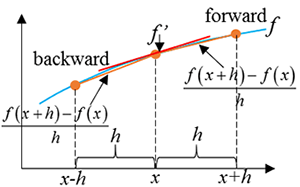
\includegraphics{finitediff.png}
\caption{finitediff.png}
\end{figure}

A similar thing can be done for second-order derivatives:
\begin{equation}
f^{\prime\prime}(x) \approx \frac{\delta_h^2 \lbrack f\rbrack (x)}{h^2} = \frac{f(x+h)-2f(x)+f(x-h)}{h^2}
\end{equation}

When the function is unknown and the data is in the form of
\((x_i,y_i)\) coordinate pairs, we can use the following as an
approximation for the second derivative:

\begin{equation}
f^{\prime\prime}(x_i) \approx \frac{y_{i+1} - 2y_i + y_{i-1}}{\left(\frac{x_{i+1}-x_{i-1}}{2}\right)^2}
\end{equation}

    \begin{tcolorbox}[breakable, size=fbox, boxrule=1pt, pad at break*=1mm,colback=cellbackground, colframe=cellborder]
\prompt{In}{incolor}{5}{\boxspacing}
\begin{Verbatim}[commandchars=\\\{\}]
\PY{k}{def} \PY{n+nf}{fin\PYZus{}diff\PYZus{}deriv}\PY{p}{(}\PY{n}{x}\PY{p}{,}\PY{n}{y}\PY{p}{,}\PY{n}{order}\PY{p}{,}\PY{n}{num\PYZus{}breaks}\PY{o}{=}\PY{l+m+mi}{3}\PY{p}{)}\PY{p}{:}
    \PY{k+kn}{from} \PY{n+nn}{scipy}\PY{n+nn}{.}\PY{n+nn}{optimize} \PY{k+kn}{import} \PY{n}{curve\PYZus{}fit}
    
    \PY{n}{logx}\PY{p}{,} \PY{n}{logy} \PY{o}{=} \PY{n}{np}\PY{o}{.}\PY{n}{log10}\PY{p}{(}\PY{n}{x}\PY{p}{)}\PY{p}{,} \PY{n}{np}\PY{o}{.}\PY{n}{log10}\PY{p}{(}\PY{n}{y}\PY{p}{)}
    
    \PY{n}{first\PYZus{}derivative} \PY{o}{=} \PY{p}{[}\PY{p}{]}
    \PY{n}{second\PYZus{}derivative} \PY{o}{=} \PY{p}{[}\PY{p}{]}
    
    \PY{k}{for} \PY{n}{idx} \PY{o+ow}{in} \PY{n+nb}{range}\PY{p}{(}\PY{l+m+mi}{1}\PY{p}{,}\PY{n+nb}{len}\PY{p}{(}\PY{n}{logx}\PY{p}{)}\PY{o}{\PYZhy{}}\PY{l+m+mi}{1}\PY{p}{)}\PY{p}{:}
        \PY{n}{first\PYZus{}derivative}\PY{o}{.}\PY{n}{append}\PY{p}{(}\PY{p}{(}\PY{n}{logy}\PY{p}{[}\PY{n}{idx}\PY{o}{+}\PY{l+m+mi}{1}\PY{p}{]} \PY{o}{\PYZhy{}} \PY{n}{logy}\PY{p}{[}\PY{n}{idx}\PY{o}{\PYZhy{}}\PY{l+m+mi}{1}\PY{p}{]}\PY{p}{)}\PY{o}{/}\PY{p}{(}\PY{n}{logx}\PY{p}{[}\PY{n}{idx}\PY{o}{+}\PY{l+m+mi}{1}\PY{p}{]}\PY{o}{\PYZhy{}}\PY{n}{logx}\PY{p}{[}\PY{n}{idx}\PY{o}{\PYZhy{}}\PY{l+m+mi}{1}\PY{p}{]}\PY{p}{)}\PY{p}{)}
        \PY{n}{second\PYZus{}derivative}\PY{o}{.}\PY{n}{append}\PY{p}{(}\PY{p}{(}\PY{n}{logy}\PY{p}{[}\PY{n}{idx}\PY{o}{+}\PY{l+m+mi}{1}\PY{p}{]} \PY{o}{\PYZhy{}} \PY{l+m+mi}{2}\PY{o}{*}\PY{n}{logy}\PY{p}{[}\PY{n}{idx}\PY{p}{]} \PY{o}{+} \PY{n}{logy}\PY{p}{[}\PY{n}{idx}\PY{o}{\PYZhy{}}\PY{l+m+mi}{1}\PY{p}{]}\PY{p}{)}\PY{o}{/}\PY{p}{(}\PY{p}{(}\PY{n}{logx}\PY{p}{[}\PY{n}{idx}\PY{o}{+}\PY{l+m+mi}{1}\PY{p}{]}\PY{o}{\PYZhy{}}\PY{n}{logx}\PY{p}{[}\PY{n}{idx}\PY{o}{\PYZhy{}}\PY{l+m+mi}{1}\PY{p}{]}\PY{p}{)}\PY{o}{/}\PY{l+m+mi}{2}\PY{p}{)}\PY{o}{*}\PY{o}{*}\PY{l+m+mi}{2}\PY{p}{)}
    
    \PY{k}{return} \PY{p}{[}\PY{n}{logy}\PY{p}{,}\PY{n}{first\PYZus{}derivative}\PY{p}{,}\PY{n}{second\PYZus{}derivative}\PY{p}{]}\PY{p}{[}\PY{n}{order}\PY{p}{]} \PY{c+c1}{\PYZsh{} placeholder for debugging: just return numerical derivative rather than anything real, for the moment}
\end{Verbatim}
\end{tcolorbox}

    \hypertarget{signal-processing-and-smoothing}{%
\subsubsection{Signal processing and
smoothing}\label{signal-processing-and-smoothing}}

Noisy and non-smooth data present a big problem for numerical
differentiation techniques.
\href{http://downloads.hindawi.com/archive/2011/164564.pdf}{Chartrand
(2011)} presents some signal-processing-type solutions. A naïve
quick-fix would be to use a rolling mean to smooth the sample. We can
also implement a low-pass filter to try to remove some of the noise
while preserving the shape of the data.

    \begin{tcolorbox}[breakable, size=fbox, boxrule=1pt, pad at break*=1mm,colback=cellbackground, colframe=cellborder]
\prompt{In}{incolor}{6}{\boxspacing}
\begin{Verbatim}[commandchars=\\\{\}]
\PY{k+kn}{from} \PY{n+nn}{scipy}\PY{n+nn}{.}\PY{n+nn}{signal} \PY{k+kn}{import} \PY{n}{savgol\PYZus{}filter}\PY{p}{,} \PY{n}{fftconvolve}

\PY{n}{smoothed} \PY{o}{=} \PY{n}{savgol\PYZus{}filter}\PY{p}{(}\PY{n}{noisy}\PY{p}{,} \PY{l+m+mi}{15}\PY{p}{,} \PY{l+m+mi}{5}\PY{p}{)} \PY{c+c1}{\PYZsh{} see § \PYZsq{}Savitzky\PYZhy{}Golay filtering\PYZsq{} below}
\PY{n}{smoothed} \PY{o}{=} \PY{n}{savgol\PYZus{}filter}\PY{p}{(}\PY{n}{smoothed}\PY{p}{,}\PY{l+m+mi}{11}\PY{p}{,}\PY{l+m+mi}{3}\PY{p}{)} \PY{c+c1}{\PYZsh{} second pass}

\PY{n}{plt}\PY{o}{.}\PY{n}{loglog}\PY{p}{(}\PY{n}{x}\PY{p}{,}\PY{n}{noisy}\PY{p}{)}
\PY{n}{plt}\PY{o}{.}\PY{n}{loglog}\PY{p}{(}\PY{n}{x}\PY{p}{,}\PY{n}{smoothed}\PY{p}{)}
\PY{n}{plt}\PY{o}{.}\PY{n}{show}\PY{p}{(}\PY{p}{)}
\end{Verbatim}
\end{tcolorbox}

    \begin{center}
    \adjustimage{max size={0.9\linewidth}{0.9\paperheight}}{brokepl_files/brokepl_9_0.png}
    \end{center}
    { \hspace*{\fill} } 
\begin{tcolorbox}[breakable, size=fbox, boxrule=1pt, pad at break*=1mm,colback=cellbackground, colframe=cellborder]
\prompt{In}{incolor}{7}{\boxspacing}
\begin{Verbatim}[commandchars=\\\{\}]
\PY{n}{labels} \PY{o}{=} \PY{n+nb}{iter}\PY{p}{(}\PY{p}{[}\PY{l+s+sa}{r}\PY{l+s+s1}{\PYZsq{}}\PY{l+s+s1}{\PYZdl{}}\PY{l+s+s1}{\PYZbs{}}\PY{l+s+s1}{nu\PYZus{}a\PYZdl{}}\PY{l+s+s1}{\PYZsq{}}\PY{p}{,}\PY{l+s+sa}{r}\PY{l+s+s1}{\PYZsq{}}\PY{l+s+s1}{\PYZdl{}}\PY{l+s+s1}{\PYZbs{}}\PY{l+s+s1}{nu\PYZus{}m\PYZdl{}}\PY{l+s+s1}{\PYZsq{}}\PY{p}{,}\PY{l+s+sa}{r}\PY{l+s+s1}{\PYZsq{}}\PY{l+s+s1}{\PYZdl{}}\PY{l+s+s1}{\PYZbs{}}\PY{l+s+s1}{nu\PYZus{}c\PYZdl{}}\PY{l+s+s1}{\PYZsq{}}\PY{p}{]}\PY{p}{)}
\PY{n}{colors} \PY{o}{=} \PY{n+nb}{iter}\PY{p}{(}\PY{l+s+s1}{\PYZsq{}}\PY{l+s+s1}{rgb}\PY{l+s+s1}{\PYZsq{}}\PY{p}{)}
\PY{n}{plt}\PY{o}{.}\PY{n}{plot}\PY{p}{(}\PY{n}{np}\PY{o}{.}\PY{n}{log10}\PY{p}{(}\PY{n}{x}\PY{p}{[}\PY{l+m+mi}{1}\PY{p}{:}\PY{o}{\PYZhy{}}\PY{l+m+mi}{1}\PY{p}{]}\PY{p}{)}\PY{p}{,}\PY{n}{fit\PYZus{}bkn\PYZus{}pow}\PY{p}{(}\PY{n}{x}\PY{p}{,}\PY{n}{noisy}\PY{p}{,}\PY{l+m+mi}{1}\PY{p}{)}\PY{p}{,}\PY{l+s+s2}{\PYZdq{}}\PY{l+s+s2}{.}\PY{l+s+s2}{\PYZdq{}}\PY{p}{)}
\PY{n}{plt}\PY{o}{.}\PY{n}{plot}\PY{p}{(}\PY{n}{np}\PY{o}{.}\PY{n}{log10}\PY{p}{(}\PY{n}{x}\PY{p}{[}\PY{l+m+mi}{1}\PY{p}{:}\PY{o}{\PYZhy{}}\PY{l+m+mi}{1}\PY{p}{]}\PY{p}{)}\PY{p}{,}\PY{n}{fit\PYZus{}bkn\PYZus{}pow}\PY{p}{(}\PY{n}{x}\PY{p}{,}\PY{n}{y}\PY{p}{,}\PY{l+m+mi}{1}\PY{p}{)}\PY{p}{,}\PY{l+s+s2}{\PYZdq{}}\PY{l+s+s2}{\PYZhy{}\PYZhy{}}\PY{l+s+s2}{\PYZdq{}}\PY{p}{)}
\PY{n}{plt}\PY{o}{.}\PY{n}{plot}\PY{p}{(}\PY{n}{np}\PY{o}{.}\PY{n}{log10}\PY{p}{(}\PY{n}{x}\PY{p}{[}\PY{l+m+mi}{1}\PY{p}{:}\PY{o}{\PYZhy{}}\PY{l+m+mi}{1}\PY{p}{]}\PY{p}{)}\PY{p}{,}\PY{n}{fit\PYZus{}bkn\PYZus{}pow}\PY{p}{(}\PY{n}{x}\PY{p}{,}\PY{n}{smoothed}\PY{p}{,}\PY{l+m+mi}{1}\PY{p}{)}\PY{p}{)}
\PY{c+c1}{\PYZsh{}plt.plot(np.log10(x),np.log10(savgol\PYZus{}filter(noisy,25,4,deriv=1)))}
\PY{k}{for} \PY{n}{br} \PY{o+ow}{in} \PY{n}{breaks}\PY{p}{:}
\PY{n}{plt}\PY{o}{.}\PY{n}{axvline}\PY{p}{(}\PY{n}{np}\PY{o}{.}\PY{n}{log10}\PY{p}{(}\PY{n}{br}\PY{p}{)}\PY{p}{,}\PY{n}{linestyle}\PY{o}{=}\PY{l+s+s2}{\PYZdq{}}\PY{l+s+s2}{\PYZhy{}\PYZhy{}}\PY{l+s+s2}{\PYZdq{}}\PY{p}{,}\PY{n}{lw}\PY{o}{=}\PY{l+m+mi}{1}\PY{p}{,}\PY{n}{color}\PY{o}{=}\PY{n+nb}{next}\PY{p}{(}\PY{n}{colors}\PY{p}{)}\PY{p}{,}\PY{n}{label}\PY{o}{=}\PY{n+nb}{next}\PY{p}{(}\PY{n}{labels}\PY{p}{)}\PY{p}{)}
\end{Verbatim}
\end{tcolorbox}
    \begin{center}
    \adjustimage{max size={0.9\linewidth}{0.9\paperheight}}{brokepl_files/brokepl_10_0.png}
    \end{center}
    { \hspace*{\fill} \\} 
    \hypertarget{savitzky-golay-filtering}{%
\paragraph{Savitzky-Golay filtering}\label{savitzky-golay-filtering}}

Savitzky-Golay is a type of low-pass filter, particularly suited for
smoothing data with high-frequency noise. The main idea behind this
approach is to make for each point a least-square fit with a polynomial
of high order over a odd-sized window centered at the point. It has the
advantage of preserving the original shape and features of the signal
better than other types of filtering approaches, such as moving average
techniques.
There is actually already a SciPy function that implements this filter: \href{https://docs.scipy.org/doc/scipy/reference/generated/scipy.signal.savgol_filter.html}{\texttt{scipy.signal.savgol\_filter}} (as already seen above). I've rewritten it below because it's not that complicated and it's worth seeing how it works. As input, it takes the noisy data, the filter window size (odd positive integer), the polynomial order to use when filtering, and the order of the derivative to compute (default \(0\) will denoise original function only). It outputs smoothed \(y\)-points. Example:
\begin{Shaded}
\begin{Highlighting}[]
\NormalTok{t }\OperatorTok{=}\NormalTok{ np.linspace(}\OperatorTok{{-}}\DecValTok{4}\NormalTok{, }\DecValTok{4}\NormalTok{, }\DecValTok{500}\NormalTok{)}
\NormalTok{y }\OperatorTok{=}\NormalTok{ np.exp( }\OperatorTok{{-}}\NormalTok{t}\OperatorTok{**}\DecValTok{2}\NormalTok{ ) }\OperatorTok{+}\NormalTok{ np.random.normal(}\DecValTok{0}\NormalTok{, }\FloatTok{0.05}\NormalTok{, t.shape)}
\NormalTok{ysg }\OperatorTok{=}\NormalTok{ savitzky\_golay(y, window\_size}\OperatorTok{=}\DecValTok{31}\NormalTok{, order}\OperatorTok{=}\DecValTok{4}\NormalTok{)}
\NormalTok{plt.plot(t, y, label}\OperatorTok{=}\StringTok{\textquotesingle{}Noisy signal\textquotesingle{}}\NormalTok{)}
\NormalTok{plt.plot(t, np.exp(}\OperatorTok{{-}}\NormalTok{t}\OperatorTok{**}\DecValTok{2}\NormalTok{), }\StringTok{\textquotesingle{}k\textquotesingle{}}\NormalTok{, lw}\OperatorTok{=}\FloatTok{1.5}\NormalTok{, label}\OperatorTok{=}\StringTok{\textquotesingle{}Original signal\textquotesingle{}}\NormalTok{)}
\NormalTok{plt.plot(t, ysg, }\StringTok{\textquotesingle{}r\textquotesingle{}}\NormalTok{, label}\OperatorTok{=}\StringTok{\textquotesingle{}Filtered signal\textquotesingle{}}\NormalTok{)}
\NormalTok{plt.legend()}
\NormalTok{plt.show()}
\end{Highlighting}
\end{Shaded}

For more, see \href{https://doi.org/10.1021/ac60214a047}{Savitzky \&
Golay (1964)} and of course,
\href{http://www.cambridge.org/9780521880688}{Numerical Recipes}.

    \begin{tcolorbox}[breakable, size=fbox, boxrule=1pt, pad at break*=1mm,colback=cellbackground, colframe=cellborder]
\prompt{In}{incolor}{8}{\boxspacing}
\begin{Verbatim}[commandchars=\\\{\}]
\PY{k}{def} \PY{n+nf}{savitzky\PYZus{}golay}\PY{p}{(}\PY{n}{y}\PY{p}{,} \PY{n}{window\PYZus{}size}\PY{p}{,} \PY{n}{order}\PY{p}{,} \PY{n}{deriv}\PY{o}{=}\PY{l+m+mi}{0}\PY{p}{,} \PY{n}{rate}\PY{o}{=}\PY{l+m+mi}{1}\PY{p}{)}\PY{p}{:}

    \PY{k}{try}\PY{p}{:}
        \PY{n}{window\PYZus{}size} \PY{o}{=} \PY{n}{np}\PY{o}{.}\PY{n}{abs}\PY{p}{(}\PY{n}{np}\PY{o}{.}\PY{n}{int}\PY{p}{(}\PY{n}{window\PYZus{}size}\PY{p}{)}\PY{p}{)}
        \PY{n}{order} \PY{o}{=} \PY{n}{np}\PY{o}{.}\PY{n}{abs}\PY{p}{(}\PY{n}{np}\PY{o}{.}\PY{n}{int}\PY{p}{(}\PY{n}{order}\PY{p}{)}\PY{p}{)}
    \PY{k}{except} \PY{n+ne}{ValueError}\PY{p}{:}
        \PY{k}{raise} \PY{n+ne}{ValueError}\PY{p}{(}\PY{l+s+s2}{\PYZdq{}}\PY{l+s+s2}{window\PYZus{}size and order should be integers}\PY{l+s+s2}{\PYZdq{}}\PY{p}{)}
    \PY{k}{if} \PY{n}{window\PYZus{}size} \PY{o}{\PYZpc{}} \PY{l+m+mi}{2} \PY{o}{!=} \PY{l+m+mi}{1} \PY{o+ow}{or} \PY{n}{window\PYZus{}size} \PY{o}{\PYZlt{}} \PY{l+m+mi}{1}\PY{p}{:}
        \PY{k}{raise} \PY{n+ne}{TypeError}\PY{p}{(}\PY{l+s+s2}{\PYZdq{}}\PY{l+s+s2}{window\PYZus{}size size must be positive and odd}\PY{l+s+s2}{\PYZdq{}}\PY{p}{)}
    \PY{k}{if} \PY{n}{window\PYZus{}size} \PY{o}{\PYZlt{}} \PY{n}{order} \PY{o}{+} \PY{l+m+mi}{2}\PY{p}{:}
        \PY{k}{raise} \PY{n+ne}{TypeError}\PY{p}{(}\PY{l+s+s2}{\PYZdq{}}\PY{l+s+s2}{window\PYZus{}size is too small for the polynomial}\PY{l+s+s2}{\PYZsq{}}\PY{l+s+s2}{s order}\PY{l+s+s2}{\PYZdq{}}\PY{p}{)}
        
    \PY{n}{half\PYZus{}window} \PY{o}{=} \PY{p}{(}\PY{n}{window\PYZus{}size}\PY{o}{\PYZhy{}}\PY{l+m+mi}{1}\PY{p}{)} \PY{o}{/}\PY{o}{/} \PY{l+m+mi}{2}
    
    \PY{c+c1}{\PYZsh{} precompute coefficients}
    \PY{n}{b} \PY{o}{=} \PY{n}{np}\PY{o}{.}\PY{n}{mat}\PY{p}{(}\PY{p}{[}\PY{p}{[}\PY{n}{k}\PY{o}{*}\PY{o}{*}\PY{n}{i} \PY{k}{for} \PY{n}{i} \PY{o+ow}{in} \PY{n+nb}{range}\PY{p}{(}\PY{n}{order}\PY{o}{+}\PY{l+m+mi}{1}\PY{p}{)}\PY{p}{]} \PY{k}{for} \PY{n}{k} \PY{o+ow}{in} \PY{n+nb}{range}\PY{p}{(}\PY{o}{\PYZhy{}}\PY{n}{half\PYZus{}window}\PY{p}{,} \PY{n}{half\PYZus{}window}\PY{o}{+}\PY{l+m+mi}{1}\PY{p}{)}\PY{p}{]}\PY{p}{)}
    \PY{n}{m} \PY{o}{=} \PY{n}{np}\PY{o}{.}\PY{n}{linalg}\PY{o}{.}\PY{n}{pinv}\PY{p}{(}\PY{n}{b}\PY{p}{)}\PY{o}{.}\PY{n}{A}\PY{p}{[}\PY{n}{deriv}\PY{p}{]} \PY{o}{*} \PY{n}{rate}\PY{o}{*}\PY{o}{*}\PY{n}{deriv} \PY{o}{*} \PY{n}{np}\PY{o}{.}\PY{n}{math}\PY{o}{.}\PY{n}{factorial}\PY{p}{(}\PY{n}{deriv}\PY{p}{)}
    
    \PY{c+c1}{\PYZsh{} pad the signal at the extremes with values taken from the signal itself}
    \PY{n}{firstvals} \PY{o}{=} \PY{n}{y}\PY{p}{[}\PY{l+m+mi}{0}\PY{p}{]} \PY{o}{\PYZhy{}} \PY{n}{np}\PY{o}{.}\PY{n}{abs}\PY{p}{(} \PY{n}{y}\PY{p}{[}\PY{l+m+mi}{1}\PY{p}{:}\PY{n}{half\PYZus{}window}\PY{o}{+}\PY{l+m+mi}{1}\PY{p}{]}\PY{p}{[}\PY{p}{:}\PY{p}{:}\PY{o}{\PYZhy{}}\PY{l+m+mi}{1}\PY{p}{]} \PY{o}{\PYZhy{}} \PY{n}{y}\PY{p}{[}\PY{l+m+mi}{0}\PY{p}{]} \PY{p}{)}
    \PY{n}{lastvals} \PY{o}{=} \PY{n}{y}\PY{p}{[}\PY{o}{\PYZhy{}}\PY{l+m+mi}{1}\PY{p}{]} \PY{o}{+} \PY{n}{np}\PY{o}{.}\PY{n}{abs}\PY{p}{(}\PY{n}{y}\PY{p}{[}\PY{o}{\PYZhy{}}\PY{n}{half\PYZus{}window}\PY{o}{\PYZhy{}}\PY{l+m+mi}{1}\PY{p}{:}\PY{o}{\PYZhy{}}\PY{l+m+mi}{1}\PY{p}{]}\PY{p}{[}\PY{p}{:}\PY{p}{:}\PY{o}{\PYZhy{}}\PY{l+m+mi}{1}\PY{p}{]} \PY{o}{\PYZhy{}} \PY{n}{y}\PY{p}{[}\PY{o}{\PYZhy{}}\PY{l+m+mi}{1}\PY{p}{]}\PY{p}{)}
    \PY{n}{y} \PY{o}{=} \PY{n}{np}\PY{o}{.}\PY{n}{concatenate}\PY{p}{(}\PY{p}{(}\PY{n}{firstvals}\PY{p}{,} \PY{n}{y}\PY{p}{,} \PY{n}{lastvals}\PY{p}{)}\PY{p}{)}
    
    \PY{k}{return} \PY{n}{np}\PY{o}{.}\PY{n}{convolve}\PY{p}{(} \PY{n}{m}\PY{p}{[}\PY{p}{:}\PY{p}{:}\PY{o}{\PYZhy{}}\PY{l+m+mi}{1}\PY{p}{]}\PY{p}{,} \PY{n}{y}\PY{p}{,} \PY{n}{mode}\PY{o}{=}\PY{l+s+s1}{\PYZsq{}}\PY{l+s+s1}{valid}\PY{l+s+s1}{\PYZsq{}}\PY{p}{)}
\end{Verbatim}
\end{tcolorbox}

    \begin{tcolorbox}[breakable, size=fbox, boxrule=1pt, pad at break*=1mm,colback=cellbackground, colframe=cellborder]
\prompt{In}{incolor}{21}{\boxspacing}
\begin{Verbatim}[commandchars=\\\{\}]
\PY{k}{def} \PY{n+nf}{sgolay2d}\PY{p}{(}\PY{n}{z}\PY{p}{,} \PY{n}{window\PYZus{}size}\PY{p}{,} \PY{n}{order}\PY{p}{,} \PY{n}{derivative}\PY{o}{=}\PY{k+kc}{None}\PY{p}{)}\PY{p}{:}
    
    \PY{c+c1}{\PYZsh{} number of terms in the polynomial expression}
    \PY{n}{n\PYZus{}terms} \PY{o}{=} \PY{p}{(} \PY{n}{order} \PY{o}{+} \PY{l+m+mi}{1} \PY{p}{)} \PY{o}{*} \PY{p}{(} \PY{n}{order} \PY{o}{+} \PY{l+m+mi}{2}\PY{p}{)}  \PY{o}{/} \PY{l+m+mf}{2.0}

    \PY{k}{if}  \PY{n}{window\PYZus{}size} \PY{o}{\PYZpc{}} \PY{l+m+mi}{2} \PY{o}{==} \PY{l+m+mi}{0}\PY{p}{:}
        \PY{k}{raise} \PY{n+ne}{ValueError}\PY{p}{(}\PY{l+s+s1}{\PYZsq{}}\PY{l+s+s1}{window\PYZus{}size must be odd}\PY{l+s+s1}{\PYZsq{}}\PY{p}{)}

    \PY{k}{if} \PY{n}{window\PYZus{}size}\PY{o}{*}\PY{o}{*}\PY{l+m+mi}{2} \PY{o}{\PYZlt{}} \PY{n}{n\PYZus{}terms}\PY{p}{:}
        \PY{k}{raise} \PY{n+ne}{ValueError}\PY{p}{(}\PY{l+s+s1}{\PYZsq{}}\PY{l+s+s1}{order is too high for the window size}\PY{l+s+s1}{\PYZsq{}}\PY{p}{)}

    \PY{n}{half\PYZus{}size} \PY{o}{=} \PY{n}{window\PYZus{}size} \PY{o}{/}\PY{o}{/} \PY{l+m+mi}{2}

    \PY{c+c1}{\PYZsh{} exponents of the polynomial. }
    \PY{c+c1}{\PYZsh{} p(x,y) = a0 + a1*x + a2*y + a3*x\PYZca{}2 + a4*y\PYZca{}2 + a5*x*y + ... }
    \PY{c+c1}{\PYZsh{} this line gives a list of two item tuple. Each tuple contains }
    \PY{c+c1}{\PYZsh{} the exponents of the k\PYZhy{}th term. First element of tuple is for x}
    \PY{c+c1}{\PYZsh{} second element for y.}
    \PY{c+c1}{\PYZsh{} Ex. exps = [(0,0), (1,0), (0,1), (2,0), (1,1), (0,2), ...]}
    \PY{n}{exps} \PY{o}{=} \PY{p}{[} \PY{p}{(}\PY{n}{k}\PY{o}{\PYZhy{}}\PY{n}{n}\PY{p}{,} \PY{n}{n}\PY{p}{)} \PY{k}{for} \PY{n}{k} \PY{o+ow}{in} \PY{n+nb}{range}\PY{p}{(}\PY{n}{order}\PY{o}{+}\PY{l+m+mi}{1}\PY{p}{)} \PY{k}{for} \PY{n}{n} \PY{o+ow}{in} \PY{n+nb}{range}\PY{p}{(}\PY{n}{k}\PY{o}{+}\PY{l+m+mi}{1}\PY{p}{)} \PY{p}{]}

    \PY{c+c1}{\PYZsh{} coordinates of points}
    \PY{n}{ind} \PY{o}{=} \PY{n}{np}\PY{o}{.}\PY{n}{arange}\PY{p}{(}\PY{o}{\PYZhy{}}\PY{n}{half\PYZus{}size}\PY{p}{,} \PY{n}{half\PYZus{}size}\PY{o}{+}\PY{l+m+mi}{1}\PY{p}{,} \PY{n}{dtype}\PY{o}{=}\PY{n}{np}\PY{o}{.}\PY{n}{float64}\PY{p}{)}
    \PY{n}{dx} \PY{o}{=} \PY{n}{np}\PY{o}{.}\PY{n}{repeat}\PY{p}{(} \PY{n}{ind}\PY{p}{,} \PY{n}{window\PYZus{}size} \PY{p}{)}
    \PY{n}{dy} \PY{o}{=} \PY{n}{np}\PY{o}{.}\PY{n}{tile}\PY{p}{(} \PY{n}{ind}\PY{p}{,} \PY{p}{[}\PY{n}{window\PYZus{}size}\PY{p}{,} \PY{l+m+mi}{1}\PY{p}{]}\PY{p}{)}\PY{o}{.}\PY{n}{reshape}\PY{p}{(}\PY{n}{window\PYZus{}size}\PY{o}{*}\PY{o}{*}\PY{l+m+mi}{2}\PY{p}{,} \PY{p}{)}

    \PY{c+c1}{\PYZsh{} build matrix of system of equation}
    \PY{n}{A} \PY{o}{=} \PY{n}{np}\PY{o}{.}\PY{n}{empty}\PY{p}{(} \PY{p}{(}\PY{n}{window\PYZus{}size}\PY{o}{*}\PY{o}{*}\PY{l+m+mi}{2}\PY{p}{,} \PY{n+nb}{len}\PY{p}{(}\PY{n}{exps}\PY{p}{)}\PY{p}{)} \PY{p}{)}
    \PY{k}{for} \PY{n}{i}\PY{p}{,} \PY{n}{exp} \PY{o+ow}{in} \PY{n+nb}{enumerate}\PY{p}{(} \PY{n}{exps} \PY{p}{)}\PY{p}{:}
        \PY{n}{A}\PY{p}{[}\PY{p}{:}\PY{p}{,}\PY{n}{i}\PY{p}{]} \PY{o}{=} \PY{p}{(}\PY{n}{dx}\PY{o}{*}\PY{o}{*}\PY{n}{exp}\PY{p}{[}\PY{l+m+mi}{0}\PY{p}{]}\PY{p}{)} \PY{o}{*} \PY{p}{(}\PY{n}{dy}\PY{o}{*}\PY{o}{*}\PY{n}{exp}\PY{p}{[}\PY{l+m+mi}{1}\PY{p}{]}\PY{p}{)}

    \PY{c+c1}{\PYZsh{} pad input array with appropriate values at the four borders}
    \PY{n}{new\PYZus{}shape} \PY{o}{=} \PY{n}{z}\PY{o}{.}\PY{n}{shape}\PY{p}{[}\PY{l+m+mi}{0}\PY{p}{]} \PY{o}{+} \PY{l+m+mi}{2}\PY{o}{*}\PY{n}{half\PYZus{}size}\PY{p}{,} \PY{n}{z}\PY{o}{.}\PY{n}{shape}\PY{p}{[}\PY{l+m+mi}{1}\PY{p}{]} \PY{o}{+} \PY{l+m+mi}{2}\PY{o}{*}\PY{n}{half\PYZus{}size}
    \PY{n}{Z} \PY{o}{=} \PY{n}{np}\PY{o}{.}\PY{n}{zeros}\PY{p}{(} \PY{p}{(}\PY{n}{new\PYZus{}shape}\PY{p}{)} \PY{p}{)}
    \PY{c+c1}{\PYZsh{} top band}
    \PY{n}{band} \PY{o}{=} \PY{n}{z}\PY{p}{[}\PY{l+m+mi}{0}\PY{p}{,} \PY{p}{:}\PY{p}{]}
    \PY{n}{Z}\PY{p}{[}\PY{p}{:}\PY{n}{half\PYZus{}size}\PY{p}{,} \PY{n}{half\PYZus{}size}\PY{p}{:}\PY{o}{\PYZhy{}}\PY{n}{half\PYZus{}size}\PY{p}{]} \PY{o}{=}  \PY{n}{band} \PY{o}{\PYZhy{}}  \PY{n}{np}\PY{o}{.}\PY{n}{abs}\PY{p}{(} \PY{n}{np}\PY{o}{.}\PY{n}{flipud}\PY{p}{(} \PY{n}{z}\PY{p}{[}\PY{l+m+mi}{1}\PY{p}{:}\PY{n}{half\PYZus{}size}\PY{o}{+}\PY{l+m+mi}{1}\PY{p}{,} \PY{p}{:}\PY{p}{]} \PY{p}{)} \PY{o}{\PYZhy{}} \PY{n}{band} \PY{p}{)}
    \PY{c+c1}{\PYZsh{} bottom band}
    \PY{n}{band} \PY{o}{=} \PY{n}{z}\PY{p}{[}\PY{o}{\PYZhy{}}\PY{l+m+mi}{1}\PY{p}{,} \PY{p}{:}\PY{p}{]}
    \PY{n}{Z}\PY{p}{[}\PY{o}{\PYZhy{}}\PY{n}{half\PYZus{}size}\PY{p}{:}\PY{p}{,} \PY{n}{half\PYZus{}size}\PY{p}{:}\PY{o}{\PYZhy{}}\PY{n}{half\PYZus{}size}\PY{p}{]} \PY{o}{=} \PY{n}{band}  \PY{o}{+} \PY{n}{np}\PY{o}{.}\PY{n}{abs}\PY{p}{(} \PY{n}{np}\PY{o}{.}\PY{n}{flipud}\PY{p}{(} \PY{n}{z}\PY{p}{[}\PY{o}{\PYZhy{}}\PY{n}{half\PYZus{}size}\PY{o}{\PYZhy{}}\PY{l+m+mi}{1}\PY{p}{:}\PY{o}{\PYZhy{}}\PY{l+m+mi}{1}\PY{p}{,} \PY{p}{:}\PY{p}{]} \PY{p}{)}  \PY{o}{\PYZhy{}}\PY{n}{band} \PY{p}{)}
    \PY{c+c1}{\PYZsh{} left band}
    \PY{n}{band} \PY{o}{=} \PY{n}{np}\PY{o}{.}\PY{n}{tile}\PY{p}{(} \PY{n}{z}\PY{p}{[}\PY{p}{:}\PY{p}{,}\PY{l+m+mi}{0}\PY{p}{]}\PY{o}{.}\PY{n}{reshape}\PY{p}{(}\PY{o}{\PYZhy{}}\PY{l+m+mi}{1}\PY{p}{,}\PY{l+m+mi}{1}\PY{p}{)}\PY{p}{,} \PY{p}{[}\PY{l+m+mi}{1}\PY{p}{,}\PY{n}{half\PYZus{}size}\PY{p}{]}\PY{p}{)}
    \PY{n}{Z}\PY{p}{[}\PY{n}{half\PYZus{}size}\PY{p}{:}\PY{o}{\PYZhy{}}\PY{n}{half\PYZus{}size}\PY{p}{,} \PY{p}{:}\PY{n}{half\PYZus{}size}\PY{p}{]} \PY{o}{=} \PY{n}{band} \PY{o}{\PYZhy{}} \PY{n}{np}\PY{o}{.}\PY{n}{abs}\PY{p}{(} \PY{n}{np}\PY{o}{.}\PY{n}{fliplr}\PY{p}{(} \PY{n}{z}\PY{p}{[}\PY{p}{:}\PY{p}{,} \PY{l+m+mi}{1}\PY{p}{:}\PY{n}{half\PYZus{}size}\PY{o}{+}\PY{l+m+mi}{1}\PY{p}{]} \PY{p}{)} \PY{o}{\PYZhy{}} \PY{n}{band} \PY{p}{)}
    \PY{c+c1}{\PYZsh{} right band}
    \PY{n}{band} \PY{o}{=} \PY{n}{np}\PY{o}{.}\PY{n}{tile}\PY{p}{(} \PY{n}{z}\PY{p}{[}\PY{p}{:}\PY{p}{,}\PY{o}{\PYZhy{}}\PY{l+m+mi}{1}\PY{p}{]}\PY{o}{.}\PY{n}{reshape}\PY{p}{(}\PY{o}{\PYZhy{}}\PY{l+m+mi}{1}\PY{p}{,}\PY{l+m+mi}{1}\PY{p}{)}\PY{p}{,} \PY{p}{[}\PY{l+m+mi}{1}\PY{p}{,}\PY{n}{half\PYZus{}size}\PY{p}{]} \PY{p}{)}
    \PY{n}{Z}\PY{p}{[}\PY{n}{half\PYZus{}size}\PY{p}{:}\PY{o}{\PYZhy{}}\PY{n}{half\PYZus{}size}\PY{p}{,} \PY{o}{\PYZhy{}}\PY{n}{half\PYZus{}size}\PY{p}{:}\PY{p}{]} \PY{o}{=}  \PY{n}{band} \PY{o}{+} \PY{n}{np}\PY{o}{.}\PY{n}{abs}\PY{p}{(} \PY{n}{np}\PY{o}{.}\PY{n}{fliplr}\PY{p}{(} \PY{n}{z}\PY{p}{[}\PY{p}{:}\PY{p}{,} \PY{o}{\PYZhy{}}\PY{n}{half\PYZus{}size}\PY{o}{\PYZhy{}}\PY{l+m+mi}{1}\PY{p}{:}\PY{o}{\PYZhy{}}\PY{l+m+mi}{1}\PY{p}{]} \PY{p}{)} \PY{o}{\PYZhy{}} \PY{n}{band} \PY{p}{)}
    \PY{c+c1}{\PYZsh{} central band}
    \PY{n}{Z}\PY{p}{[}\PY{n}{half\PYZus{}size}\PY{p}{:}\PY{o}{\PYZhy{}}\PY{n}{half\PYZus{}size}\PY{p}{,} \PY{n}{half\PYZus{}size}\PY{p}{:}\PY{o}{\PYZhy{}}\PY{n}{half\PYZus{}size}\PY{p}{]} \PY{o}{=} \PY{n}{z}

    \PY{c+c1}{\PYZsh{} top left corner}
    \PY{n}{band} \PY{o}{=} \PY{n}{z}\PY{p}{[}\PY{l+m+mi}{0}\PY{p}{,}\PY{l+m+mi}{0}\PY{p}{]}
    \PY{n}{Z}\PY{p}{[}\PY{p}{:}\PY{n}{half\PYZus{}size}\PY{p}{,}\PY{p}{:}\PY{n}{half\PYZus{}size}\PY{p}{]} \PY{o}{=} \PY{n}{band} \PY{o}{\PYZhy{}} \PY{n}{np}\PY{o}{.}\PY{n}{abs}\PY{p}{(} \PY{n}{np}\PY{o}{.}\PY{n}{flipud}\PY{p}{(}\PY{n}{np}\PY{o}{.}\PY{n}{fliplr}\PY{p}{(}\PY{n}{z}\PY{p}{[}\PY{l+m+mi}{1}\PY{p}{:}\PY{n}{half\PYZus{}size}\PY{o}{+}\PY{l+m+mi}{1}\PY{p}{,}\PY{l+m+mi}{1}\PY{p}{:}\PY{n}{half\PYZus{}size}\PY{o}{+}\PY{l+m+mi}{1}\PY{p}{]}\PY{p}{)} \PY{p}{)} \PY{o}{\PYZhy{}} \PY{n}{band} \PY{p}{)}
    \PY{c+c1}{\PYZsh{} bottom right corner}
    \PY{n}{band} \PY{o}{=} \PY{n}{z}\PY{p}{[}\PY{o}{\PYZhy{}}\PY{l+m+mi}{1}\PY{p}{,}\PY{o}{\PYZhy{}}\PY{l+m+mi}{1}\PY{p}{]}
    \PY{n}{Z}\PY{p}{[}\PY{o}{\PYZhy{}}\PY{n}{half\PYZus{}size}\PY{p}{:}\PY{p}{,}\PY{o}{\PYZhy{}}\PY{n}{half\PYZus{}size}\PY{p}{:}\PY{p}{]} \PY{o}{=} \PY{n}{band} \PY{o}{+} \PY{n}{np}\PY{o}{.}\PY{n}{abs}\PY{p}{(} \PY{n}{np}\PY{o}{.}\PY{n}{flipud}\PY{p}{(}\PY{n}{np}\PY{o}{.}\PY{n}{fliplr}\PY{p}{(}\PY{n}{z}\PY{p}{[}\PY{o}{\PYZhy{}}\PY{n}{half\PYZus{}size}\PY{o}{\PYZhy{}}\PY{l+m+mi}{1}\PY{p}{:}\PY{o}{\PYZhy{}}\PY{l+m+mi}{1}\PY{p}{,}\PY{o}{\PYZhy{}}\PY{n}{half\PYZus{}size}\PY{o}{\PYZhy{}}\PY{l+m+mi}{1}\PY{p}{:}\PY{o}{\PYZhy{}}\PY{l+m+mi}{1}\PY{p}{]}\PY{p}{)} \PY{p}{)} \PY{o}{\PYZhy{}} \PY{n}{band} \PY{p}{)}

    \PY{c+c1}{\PYZsh{} top right corner}
    \PY{n}{band} \PY{o}{=} \PY{n}{Z}\PY{p}{[}\PY{n}{half\PYZus{}size}\PY{p}{,}\PY{o}{\PYZhy{}}\PY{n}{half\PYZus{}size}\PY{p}{:}\PY{p}{]}
    \PY{n}{Z}\PY{p}{[}\PY{p}{:}\PY{n}{half\PYZus{}size}\PY{p}{,}\PY{o}{\PYZhy{}}\PY{n}{half\PYZus{}size}\PY{p}{:}\PY{p}{]} \PY{o}{=} \PY{n}{band} \PY{o}{\PYZhy{}} \PY{n}{np}\PY{o}{.}\PY{n}{abs}\PY{p}{(} \PY{n}{np}\PY{o}{.}\PY{n}{flipud}\PY{p}{(}\PY{n}{Z}\PY{p}{[}\PY{n}{half\PYZus{}size}\PY{o}{+}\PY{l+m+mi}{1}\PY{p}{:}\PY{l+m+mi}{2}\PY{o}{*}\PY{n}{half\PYZus{}size}\PY{o}{+}\PY{l+m+mi}{1}\PY{p}{,}\PY{o}{\PYZhy{}}\PY{n}{half\PYZus{}size}\PY{p}{:}\PY{p}{]}\PY{p}{)} \PY{o}{\PYZhy{}} \PY{n}{band} \PY{p}{)}
    \PY{c+c1}{\PYZsh{} bottom left corner}
    \PY{n}{band} \PY{o}{=} \PY{n}{Z}\PY{p}{[}\PY{o}{\PYZhy{}}\PY{n}{half\PYZus{}size}\PY{p}{:}\PY{p}{,}\PY{n}{half\PYZus{}size}\PY{p}{]}\PY{o}{.}\PY{n}{reshape}\PY{p}{(}\PY{o}{\PYZhy{}}\PY{l+m+mi}{1}\PY{p}{,}\PY{l+m+mi}{1}\PY{p}{)}
    \PY{n}{Z}\PY{p}{[}\PY{o}{\PYZhy{}}\PY{n}{half\PYZus{}size}\PY{p}{:}\PY{p}{,}\PY{p}{:}\PY{n}{half\PYZus{}size}\PY{p}{]} \PY{o}{=} \PY{n}{band} \PY{o}{\PYZhy{}} \PY{n}{np}\PY{o}{.}\PY{n}{abs}\PY{p}{(} \PY{n}{np}\PY{o}{.}\PY{n}{fliplr}\PY{p}{(}\PY{n}{Z}\PY{p}{[}\PY{o}{\PYZhy{}}\PY{n}{half\PYZus{}size}\PY{p}{:}\PY{p}{,} \PY{n}{half\PYZus{}size}\PY{o}{+}\PY{l+m+mi}{1}\PY{p}{:}\PY{l+m+mi}{2}\PY{o}{*}\PY{n}{half\PYZus{}size}\PY{o}{+}\PY{l+m+mi}{1}\PY{p}{]}\PY{p}{)} \PY{o}{\PYZhy{}} \PY{n}{band} \PY{p}{)}

    \PY{c+c1}{\PYZsh{} solve system and convolve}
    \PY{k}{if} \PY{n}{derivative} \PY{o}{==} \PY{k+kc}{None}\PY{p}{:}
        \PY{n}{m} \PY{o}{=} \PY{n}{np}\PY{o}{.}\PY{n}{linalg}\PY{o}{.}\PY{n}{pinv}\PY{p}{(}\PY{n}{A}\PY{p}{)}\PY{p}{[}\PY{l+m+mi}{0}\PY{p}{]}\PY{o}{.}\PY{n}{reshape}\PY{p}{(}\PY{p}{(}\PY{n}{window\PYZus{}size}\PY{p}{,} \PY{o}{\PYZhy{}}\PY{l+m+mi}{1}\PY{p}{)}\PY{p}{)}
        \PY{k}{return} \PY{n}{fftconvolve}\PY{p}{(}\PY{n}{Z}\PY{p}{,} \PY{n}{m}\PY{p}{,} \PY{n}{mode}\PY{o}{=}\PY{l+s+s1}{\PYZsq{}}\PY{l+s+s1}{valid}\PY{l+s+s1}{\PYZsq{}}\PY{p}{)}
    \PY{k}{elif} \PY{n}{derivative} \PY{o}{==} \PY{l+s+s1}{\PYZsq{}}\PY{l+s+s1}{col}\PY{l+s+s1}{\PYZsq{}}\PY{p}{:}
        \PY{n}{c} \PY{o}{=} \PY{n}{np}\PY{o}{.}\PY{n}{linalg}\PY{o}{.}\PY{n}{pinv}\PY{p}{(}\PY{n}{A}\PY{p}{)}\PY{p}{[}\PY{l+m+mi}{1}\PY{p}{]}\PY{o}{.}\PY{n}{reshape}\PY{p}{(}\PY{p}{(}\PY{n}{window\PYZus{}size}\PY{p}{,} \PY{o}{\PYZhy{}}\PY{l+m+mi}{1}\PY{p}{)}\PY{p}{)}
        \PY{k}{return} \PY{n}{fftconvolve}\PY{p}{(}\PY{n}{Z}\PY{p}{,} \PY{o}{\PYZhy{}}\PY{n}{c}\PY{p}{,} \PY{n}{mode}\PY{o}{=}\PY{l+s+s1}{\PYZsq{}}\PY{l+s+s1}{valid}\PY{l+s+s1}{\PYZsq{}}\PY{p}{)}
    \PY{k}{elif} \PY{n}{derivative} \PY{o}{==} \PY{l+s+s1}{\PYZsq{}}\PY{l+s+s1}{row}\PY{l+s+s1}{\PYZsq{}}\PY{p}{:}
        \PY{n}{r} \PY{o}{=} \PY{n}{np}\PY{o}{.}\PY{n}{linalg}\PY{o}{.}\PY{n}{pinv}\PY{p}{(}\PY{n}{A}\PY{p}{)}\PY{p}{[}\PY{l+m+mi}{2}\PY{p}{]}\PY{o}{.}\PY{n}{reshape}\PY{p}{(}\PY{p}{(}\PY{n}{window\PYZus{}size}\PY{p}{,} \PY{o}{\PYZhy{}}\PY{l+m+mi}{1}\PY{p}{)}\PY{p}{)}
        \PY{k}{return} \PY{n}{fftconvolve}\PY{p}{(}\PY{n}{Z}\PY{p}{,} \PY{o}{\PYZhy{}}\PY{n}{r}\PY{p}{,} \PY{n}{mode}\PY{o}{=}\PY{l+s+s1}{\PYZsq{}}\PY{l+s+s1}{valid}\PY{l+s+s1}{\PYZsq{}}\PY{p}{)}
    \PY{k}{elif} \PY{n}{derivative} \PY{o}{==} \PY{l+s+s1}{\PYZsq{}}\PY{l+s+s1}{both}\PY{l+s+s1}{\PYZsq{}}\PY{p}{:}
        \PY{n}{c} \PY{o}{=} \PY{n}{np}\PY{o}{.}\PY{n}{linalg}\PY{o}{.}\PY{n}{pinv}\PY{p}{(}\PY{n}{A}\PY{p}{)}\PY{p}{[}\PY{l+m+mi}{1}\PY{p}{]}\PY{o}{.}\PY{n}{reshape}\PY{p}{(}\PY{p}{(}\PY{n}{window\PYZus{}size}\PY{p}{,} \PY{o}{\PYZhy{}}\PY{l+m+mi}{1}\PY{p}{)}\PY{p}{)}
        \PY{n}{r} \PY{o}{=} \PY{n}{np}\PY{o}{.}\PY{n}{linalg}\PY{o}{.}\PY{n}{pinv}\PY{p}{(}\PY{n}{A}\PY{p}{)}\PY{p}{[}\PY{l+m+mi}{2}\PY{p}{]}\PY{o}{.}\PY{n}{reshape}\PY{p}{(}\PY{p}{(}\PY{n}{window\PYZus{}size}\PY{p}{,} \PY{o}{\PYZhy{}}\PY{l+m+mi}{1}\PY{p}{)}\PY{p}{)}
        \PY{k}{return} \PY{n}{fftconvolve}\PY{p}{(}\PY{n}{Z}\PY{p}{,} \PY{o}{\PYZhy{}}\PY{n}{r}\PY{p}{,} \PY{n}{mode}\PY{o}{=}\PY{l+s+s1}{\PYZsq{}}\PY{l+s+s1}{valid}\PY{l+s+s1}{\PYZsq{}}\PY{p}{)}\PY{p}{,} \PY{n}{fftconvolve}\PY{p}{(}\PY{n}{Z}\PY{p}{,} \PY{o}{\PYZhy{}}\PY{n}{c}\PY{p}{,} \PY{n}{mode}\PY{o}{=}\PY{l+s+s1}{\PYZsq{}}\PY{l+s+s1}{valid}\PY{l+s+s1}{\PYZsq{}}\PY{p}{)}
\end{Verbatim}
\end{tcolorbox}

    \begin{tcolorbox}[breakable, size=fbox, boxrule=1pt, pad at break*=1mm,colback=cellbackground, colframe=cellborder]
\prompt{In}{incolor}{48}{\boxspacing}
\begin{Verbatim}[commandchars=\\\{\}]
\PY{c+c1}{\PYZsh{} sample 2D data}
\PY{n}{x} \PY{o}{=} \PY{n}{np}\PY{o}{.}\PY{n}{linspace}\PY{p}{(}\PY{o}{\PYZhy{}}\PY{l+m+mi}{3}\PY{p}{,}\PY{l+m+mi}{3}\PY{p}{,}\PY{l+m+mi}{100}\PY{p}{)}
\PY{n}{y} \PY{o}{=} \PY{n}{np}\PY{o}{.}\PY{n}{linspace}\PY{p}{(}\PY{o}{\PYZhy{}}\PY{l+m+mi}{3}\PY{p}{,}\PY{l+m+mi}{3}\PY{p}{,}\PY{l+m+mi}{100}\PY{p}{)}
\PY{n}{X}\PY{p}{,} \PY{n}{Y} \PY{o}{=} \PY{n}{np}\PY{o}{.}\PY{n}{meshgrid}\PY{p}{(}\PY{n}{x}\PY{p}{,}\PY{n}{y}\PY{p}{)}

\PY{n}{Z} \PY{o}{=} \PY{n}{np}\PY{o}{.}\PY{n}{exp}\PY{p}{(} \PY{o}{\PYZhy{}}\PY{p}{(}\PY{n}{X}\PY{o}{*}\PY{o}{*}\PY{l+m+mi}{2}\PY{o}{+}\PY{n}{Y}\PY{o}{*}\PY{o}{*}\PY{l+m+mi}{2}\PY{p}{)}\PY{p}{)} \PY{c+c1}{\PYZsh{} pure function}
\PY{n}{Zn} \PY{o}{=} \PY{n}{Z} \PY{o}{+} \PY{n}{np}\PY{o}{.}\PY{n}{random}\PY{o}{.}\PY{n}{normal}\PY{p}{(} \PY{l+m+mi}{0}\PY{p}{,} \PY{l+m+mf}{0.2}\PY{p}{,} \PY{n}{Z}\PY{o}{.}\PY{n}{shape} \PY{p}{)} \PY{c+c1}{\PYZsh{} added noise}
\PY{n}{Zf} \PY{o}{=} \PY{n}{sgolay2d}\PY{p}{(} \PY{n}{Zn}\PY{p}{,} \PY{n}{window\PYZus{}size}\PY{o}{=}\PY{l+m+mi}{29}\PY{p}{,} \PY{n}{order}\PY{o}{=}\PY{l+m+mi}{4}\PY{p}{)} \PY{c+c1}{\PYZsh{} re\PYZhy{}filtered}

\PY{n}{fig} \PY{o}{=} \PY{n}{plt}\PY{o}{.}\PY{n}{figure}\PY{p}{(}\PY{n}{figsize}\PY{o}{=}\PY{p}{(}\PY{l+m+mi}{12}\PY{p}{,}\PY{l+m+mi}{4}\PY{p}{)}\PY{p}{)}
\PY{n}{axs} \PY{o}{=} \PY{p}{[}\PY{n}{fig}\PY{o}{.}\PY{n}{add\PYZus{}subplot}\PY{p}{(}\PY{n}{arr}\PY{p}{)} \PY{k}{for} \PY{n}{arr} \PY{o+ow}{in} \PY{p}{[}\PY{l+m+mi}{131}\PY{p}{,}\PY{l+m+mi}{132}\PY{p}{,}\PY{l+m+mi}{133}\PY{p}{]}\PY{p}{]}

\PY{k}{for} \PY{n}{ax}\PY{p}{,}\PY{n}{mat} \PY{o+ow}{in} \PY{n+nb}{zip}\PY{p}{(}\PY{n}{axs}\PY{p}{,}\PY{p}{[}\PY{n}{Z}\PY{p}{,}\PY{n}{Zn}\PY{p}{,}\PY{n}{Zf}\PY{p}{]}\PY{p}{)}\PY{p}{:}
    \PY{n}{ax}\PY{o}{.}\PY{n}{matshow}\PY{p}{(}\PY{n}{mat}\PY{p}{)}
\PY{n}{ax}\PY{o}{.}\PY{n}{tick\PYZus{}params}\PY{p}{(}\PY{n}{axis}\PY{o}{=}\PY{l+s+s1}{\PYZsq{}}\PY{l+s+s1}{both}\PY{l+s+s1}{\PYZsq{}}\PY{p}{,}   \PY{n}{which}\PY{o}{=}\PY{l+s+s1}{\PYZsq{}}\PY{l+s+s1}{both}\PY{l+s+s1}{\PYZsq{}}\PY{p}{,}\PY{n}{bottom}\PY{o}{=}\PY{k+kc}{False}\PY{p}{,}\PY{n}{top}\PY{o}{=}\PY{k+kc}{False}\PY{p}{,}\PY{n}{left}\PY{o}{=}\PY{k+kc}{False}\PY{p}{,}\PY{n}{labeltop}\PY{o}{=}\PY{k+kc}{False}\PY{p}{,}\PY{n}{labelleft}\PY{o}{=}\PY{k+kc}{False}\PY{p}{)}
\end{Verbatim}
\end{tcolorbox}

    \begin{center}
    \adjustimage{max size={0.9\linewidth}{0.9\paperheight}}{brokepl_files/brokepl_14_0.png}
    \end{center}
    { \hspace*{\fill} } 
    \begin{tcolorbox}[breakable, size=fbox, boxrule=1pt, pad at break*=1mm,colback=cellbackground, colframe=cellborder]
\prompt{In}{incolor}{ }{\boxspacing}
\begin{Verbatim}[commandchars=\\\{\}]
\end{Verbatim}
\end{tcolorbox}


    % Add a bibliography block to the postdoc
    
    
    
\end{document}
